\documentclass[output=paper,hidelinks]{langscibook}
\ChapterDOI{10.5281/zenodo.10186054}
\title{LFG and Tree-Adjoining Grammar}
\author{Jamie Y.\ Findlay\affiliation{University of Oslo}}
\abstract{  This chapter gives an introduction to Tree-Adjoining Grammar (TAG) and draws   some comparisons with Lexical Functional Grammar (LFG). It is primarily aimed  at those familiar with LFG who are looking to learn about TAG and see where  the two formalisms differ\slash overlap, but the comparisons will also be of   interest to those coming from a TAG background. After introducing TAG, the   chapter considers questions of generative capacity, lexicalisation, and the  factoring of redundancies from grammars. It then concludes by illustrating the   potential for combining LFG and TAG, and discusses the theoretical  implications of doing so.}

\IfFileExists{../localcommands.tex}{
   \addbibresource{../localbibliography.bib}
   \addbibresource{thisvolume.bib}
   % add all extra packages you need to load to this file

\usepackage{tabularx}
\usepackage{multicol}
\usepackage{url}
\urlstyle{same}
%\usepackage{amsmath,amssymb}

% Tight underlining according to https://alexwlchan.net/2017/10/latex-underlines/
\usepackage{contour}
\usepackage[normalem]{ulem}
\renewcommand{\ULdepth}{1.8pt}
\contourlength{0.8pt}
\newcommand{\tightuline}[1]{%
  \uline{\phantom{#1}}%
  \llap{\contour{white}{#1}}}
  
\usepackage{listings}
\lstset{basicstyle=\ttfamily,tabsize=2,breaklines=true}

% \usepackage{langsci-basic}
\usepackage{langsci-optional}
\usepackage[danger]{langsci-lgr}
\usepackage{langsci-gb4e}
%\usepackage{langsci-linguex}
%\usepackage{langsci-forest-setup}
\usepackage[tikz]{langsci-avm} % added tikz flag, 29 July 21
% \usepackage{langsci-textipa}

\usepackage[linguistics,edges]{forest}
\usepackage{tikz-qtree}
\usetikzlibrary{positioning, tikzmark, arrows.meta, calc, matrix, shapes.symbols}
\usetikzlibrary{arrows, arrows.meta, shapes, chains, decorations.text}

%%%%%%%%%%%%%%%%%%%%% Packages for all chapters

% arrows and lines between structures
\usepackage{pst-node}

% lfg attributes and values, lines (relies on pst-node), lexical entries, phrase structure rules
\usepackage{packages/lfg-abbrevs}

% subfigures
\usepackage{subcaption}

% macros for small illustrations in the glossary
\usepackage{./packages/picins}

%%%%%%%%%%%%%%%%%%%%% Packages from contributors

% % Simpler Syntax packages
\usepackage{bm}
\tikzstyle{block} = [rectangle, draw, text width=5em, text centered, minimum height=3em]
\tikzstyle{line} = [draw, thick, -latex']

% Dependency packages
\usepackage{tikz-dependency}
%\usepackage{sdrt}

\usepackage{soul}

\usepackage[notipa]{ot-tableau}

% Historical
\usepackage{stackengine}
\usepackage{bigdelim}

% Morphology
\usepackage{./packages/prooftree}
\usepackage{arydshln}
\usepackage{stmaryrd}

% TAG
\usepackage{pbox}

\usepackage{langsci-branding}

   % %%%%%%%%% lang sci press commands

\newcommand*{\orcid}{}

\makeatletter
\let\thetitle\@title
\let\theauthor\@author
\makeatother

\newcommand{\togglepaper}[1][0]{
   \bibliography{../localbibliography}
   \papernote{\scriptsize\normalfont
     \theauthor.
     \titleTemp.
     To appear in:
     Dalrymple, Mary (ed.).
     Handbook of Lexical Functional Grammar.
     Berlin: Language Science Press. [preliminary page numbering]
   }
   \pagenumbering{roman}
   \setcounter{chapter}{#1}
   \addtocounter{chapter}{-1}
}

\DeclareOldFontCommand{\rm}{\normalfont\rmfamily}{\mathrm}
\DeclareOldFontCommand{\sf}{\normalfont\sffamily}{\mathsf}
\DeclareOldFontCommand{\tt}{\normalfont\ttfamily}{\mathtt}
\DeclareOldFontCommand{\bf}{\normalfont\bfseries}{\mathbf}
\DeclareOldFontCommand{\it}{\normalfont\itshape}{\mathit}
\makeatletter
\DeclareOldFontCommand{\sc}{\normalfont\scshape}{\@nomath\sc}
\makeatother

% Bug fix, 3 April 2021
\SetupAffiliations{output in groups = false,
                   separator between two = {\bigskip\\},
                   separator between multiple = {\bigskip\\},
                   separator between final two = {\bigskip\\}
                   }

% commands for all chapters
\setmathfont{LibertinusMath-Additions.otf}[range="22B8]

% punctuation between a sequence of years in a citation
% OLD: \renewcommand{\compcitedelim}{\multicitedelim}
\renewcommand{\compcitedelim}{\addcomma\space}

% \citegen with no parentheses around year
\providecommand{\citegenalt}[2][]{\citeauthor{#2}'s \citeyear*[#1]{#2}}

% avms with plain font, using langsci-avm package
\avmdefinestyle{plain}{attributes=\normalfont,values=\normalfont,types=\normalfont,extraskip=0.2em}
% avms with attributes and values in small caps, using langsci-avm package
\avmdefinestyle{fstr}{attributes=\scshape,values=\scshape,extraskip=0.2em}
% avms with attributes in small caps, values in plain font (from peter sells)
\avmdefinestyle{fstr-ps}{attributes=\scshape,values=\normalfont,extraskip=0.2em}

% reference to previous or following examples, from Stefan
%(\mex{1}) is like \next, referring to the next example
%(\mex{0}) is like \last, referring to the previous example, etc
\makeatletter
\newcommand{\mex}[1]{\the\numexpr\c@equation+#1\relax}
\makeatother

% do not add xspace before these
\xspaceaddexceptions{1234=|*\}\restrict\,}

% Several chapters use evnup -- this is verbatim from lingmacros.sty
\makeatletter
\def\evnup{\@ifnextchar[{\@evnup}{\@evnup[0pt]}}
\def\@evnup[#1]#2{\setbox1=\hbox{#2}%
\dimen1=\ht1 \advance\dimen1 by -.5\baselineskip%
\advance\dimen1 by -#1%
\leavevmode\lower\dimen1\box1}
\makeatother

% Centered entries in tables.  Requires array package.
\newcolumntype{P}[1]{>{\centering\arraybackslash}p{#1}}

% Reference to multiple figures, requested by Victoria Rosen
\newcommand{\figsref}[2]{Figures~\ref{#1}~and~\ref{#2}}
\newcommand{\figsrefthree}[3]{Figures~\ref{#1},~\ref{#2}~and~\ref{#3}}
\newcommand{\figsreffour}[4]{Figures~\ref{#1},~\ref{#2},~\ref{#3}~and~\ref{#4}}
\newcommand{\figsreffive}[5]{Figures~\ref{#1},~\ref{#2},~\ref{#3},~\ref{#4}~and~\ref{#5}}

% Semitic chapter:
\providecommand{\textchi}{χ}

% Prosody chapter
\makeatletter
\providecommand{\leftleadsto}{%
  \mathrel{\mathpalette\reflect@squig\relax}%
}
\newcommand{\reflect@squig}[2]{%
  \reflectbox{$\m@th#1$$\leadsto$}%
}
\makeatother
\newcommand\myrotaL[1]{\mathrel{\rotatebox[origin=c]{#1}{$\leadsto$}}}
\newcommand\Prosleftarrow{\myrotaL{-135}}
\newcommand\myrotaR[1]{\mathrel{\rotatebox[origin=c]{#1}{$\leftleadsto$}}}
\newcommand\Prosrightarrow{\myrotaR{135}}

% Core Concepts chapter
\newcommand{\anterm}[2]{#1\\#2}
\newcommand{\annode}[2]{#1\\#2}

% HPSG chapter
\newcommand{\HPSGphon}[1]{〈#1〉}
% for defining RSRL relations:
\newcommand{\HPSGsfl}{\enskip\ensuremath{\stackrel{\forall{}}{\Longleftarrow{}}}\enskip}
% AVM commands, valid only inside \avm{}
\avmdefinecommand {phon}[phon] { attributes=\itshape } % define a new \phon command
% Forest Set-up
\forestset
  {notin label above/.style={edge label={node[midway,sloped,above,inner sep=0pt]{\strut$\ni$}}},
    notin label below/.style={edge label={node[midway,sloped,below,inner sep=0pt]{\strut$\ni$}}},
  }

% Dependency chapter
\newcommand{\ua}{\ensuremath{\uparrow}}
\newcommand{\da}{\ensuremath{\downarrow}}
\forestset{
  dg edges/.style={for tree={parent anchor=south, child anchor=north,align=center,base=bottom},
                 where n children=0{tier=word,edge=dotted,calign with current edge}{}
                },
dg transfer/.style={edge path={\noexpand\path[\forestoption{edge}, rounded corners=3pt]
    % the line downwards
    (!u.parent anchor)-- +($(0,-l)-(0,4pt)$)-- +($(12pt,-l)-(0,4pt)$)
    % the horizontal line
    ($(!p.north west)+(0,l)-(0,20pt)$)--($(.north east)+(0,l)-(0,20pt)$)\forestoption{edge label};},!p.edge'={}},
% for Tesniere-style junctions
dg junction/.style={no edge, tikz+={\draw (!p.east)--(!.west) (.east)--(!n.west);}    }
}


% Glossary
\makeatletter % does not work with \newcommand
\def\namedlabel#1#2{\begingroup
   \def\@currentlabel{#2}%
   \phantomsection\label{#1}\endgroup
}
\makeatother


\renewcommand{\textopeno}{ɔ}
\providecommand{\textepsilon}{ɛ}

\renewcommand{\textbari}{ɨ}
\renewcommand{\textbaru}{ʉ}
\newcommand{\acutetextbari}{í̵}
\renewcommand{\textlyoghlig}{ɮ}
\renewcommand{\textdyoghlig}{ʤ}
\renewcommand{\textschwa}{ə}
\renewcommand{\textprimstress}{ˈ}
\newcommand{\texteng}{ŋ}
\renewcommand{\textbeltl}{ɬ}
\newcommand{\textramshorns}{ɤ}

\newbool{bookcompile}
\booltrue{bookcompile}
\newcommand{\bookorchapter}[2]{\ifbool{bookcompile}{#1}{#2}}




\renewcommand{\textsci}{ɪ}
\renewcommand{\textturnscripta}{ɒ}

\renewcommand{\textscripta}{ɑ}
\renewcommand{\textteshlig}{ʧ}
\providecommand{\textupsilon}{υ}
\renewcommand{\textyogh}{ʒ}
\newcommand{\textpolhook}{̨}

\renewcommand{\sectref}[1]{Section~\ref{#1}}

%\KOMAoptions{chapterprefix=true}

\renewcommand{\textturnv}{ʌ}
\renewcommand{\textrevepsilon}{ɜ}
\renewcommand{\textsecstress}{ˌ}
\renewcommand{\textscriptv}{ʋ}
\renewcommand{\textglotstop}{ʔ}
\renewcommand{\textrevglotstop}{ʕ}
%\newcommand{\textcrh}{ħ}
\renewcommand{\textesh}{ʃ}

% label for submitted and published chapters
\newcommand{\submitted}{{\color{red}Final version submitted to Language Science Press.}}
\newcommand{\published}{{\color{red}Final version published by
    Language Science Press, available at \url{https://langsci-press.org/catalog/book/312}.}}

% Treebank definitions
\definecolor{tomato}{rgb}{0.9,0,0}
\definecolor{kelly}{rgb}{0,0.65,0}

% Minimalism chapter
\newcommand\tr[1]{$<$\textcolor{gray}{#1}$>$}
\newcommand\gapline{\lower.1ex\hbox to 1.2em{\bf \ \hrulefill\ }}
\newcommand\cnom{{\llap{[}}Case:Nom{\rlap{]}}}
\newcommand\cacc{{\llap{[}}Case:Acc{\rlap{]}}}
\newcommand\tpres{{\llap{[}}Tns:Pres{\rlap{]}}}
\newcommand\fstackwe{{\llap{[}}Tns:Pres{\rlap{]}}\\{\llap{[}}Pers:1{\rlap{]}}\\{\llap{[}}Num:Pl{\rlap{]}}}
\newcommand\fstackone{{\llap{[}}Tns:Past{\rlap{]}}\\{\llap{[}}Pers:\ {\rlap{]}}\\{\llap{[}}Num:\ {\rlap{]}}}
\newcommand\fstacktwo{{\llap{[}}Pers:3{\rlap{]}}\\{\llap{[}}Num:Pl{\rlap{]}}\\{\llap{[}}Case:\ {\rlap{]}}}
\newcommand\fstackthr{{\llap{[}}Tns:Past{\rlap{]}}\\{\llap{[}}Pers:3{\rlap{]}}\\{\llap{[}}Num:Pl{\rlap{]}}} 
\newcommand\fstackfou{{\llap{[}}Pers:3{\rlap{]}}\\{\llap{[}}Num:Pl{\rlap{]}}\\{\llap{[}}Case:Nom{\rlap{]}}}
\newcommand\fstackonefill{{\llap{[}}Tns:Past{\rlap{]}}\\{\llap{[}}Pers:3{\rlap{]}}\\%
  {\llap{[}}Num:Pl{\rlap{]}}}
\newcommand\fstackoneint%
    {{\llap{[}}{\bf Tns:Past}{\rlap{]}}\\{\llap{[}}Pers:\ {\rlap{]}}\\{\llap{[}}Num:\ {\rlap{]}}}
\newcommand\fstacktwoint%
    {{\llap{[}}{\bf Pers:3}{\rlap{]}}\\{\llap{[}}{\bf Num:Pl}{\rlap{]}}\\{\llap{[}}Case:\ {\rlap{]}}}
\newcommand\fstackthrchk%
    {{\llap{[}}{\bf Tns:Past}{\rlap{]}}\\{\llap{[}}{Pers:3}{\rlap{]}}\\%
      {\llap{[}}Num:Pl{\rlap{]}}} 
\newcommand\fstackfouchk%
    {{\llap{[}}{\bf Pers:3}{\rlap{]}}\\{\llap{[}}{\bf Num:Pl}{\rlap{]}}\\%
      {\llap{[}}Case:Nom{\rlap{]}}}
\newcommand\uinfl{{\llap{[}}Infl:\ \ {\rlap{]}}}
\newcommand\inflpass{{\llap{[}}Infl:Pass{\rlap{]}}}
\newcommand\fepp{{\llap{[}}EPP{\rlap{]}}}
\newcommand\sepp{{\llap{[}}\st{EPP}{\rlap{]}}}
\newcommand\rdash{\rlap{\hbox to 24em{\hfill (dashed lines represent
      information flow)}}}


% Computational chapter
\usepackage{./packages/kaplan}
\renewcommand{\red}{\color{lsLightWine}}

% Sinitic
\newcommand{\FRAME}{\textsc{frame}\xspace}
\newcommand{\arglistit}[1]{{\textlangle}\textit{#1}{\textrangle}}

%WestGermanic
\newcommand{\streep}[1]{\mbox{\rule{1pt}{0pt}\rule[.5ex]{#1}{.5pt}\rule{-1pt}{0pt}\rule{-#1}{0pt}}}

\newcommand{\hspaceThis}[1]{\hphantom{#1}}


\newcommand{\FIG}{\textsc{figure}}
\newcommand{\GR}{\textsc{ground}}

%%%%% Morphology
% Single quote
\newcommand{\asquote}[1]{`{#1}'} % Single quotes
\newcommand{\atrns}[1]{\asquote{#1}} % Translation
\newcommand{\attrns}[1]{(\asquote{#1})} % Translation
\newcommand{\ascare}[1]{\asquote{#1}} % Scare quotes
\newcommand{\aqterm}[1]{\asquote{#1}} % Quoted terms
% Double quote
\newcommand{\adquote}[1]{``{#1}''} % Double quotes
\newcommand{\aquoot}[1]{\adquote{#1}} % Quotes
% Italics
\newcommand{\aword}[1]{\textit{#1}}  % mention of word
\newcommand{\aterm}[1]{\textit{#1}}
% Small caps
\newcommand{\amg}[1]{{\textsc{\MakeLowercase{#1}}}}
\newcommand{\ali}[1]{\MakeLowercase{\textsc{#1}}}
\newcommand{\feat}[1]{{\textsc{#1}}}
\newcommand{\val}[1]{\textsc{#1}}
\newcommand{\pred}[1]{\textsc{#1}}
\newcommand{\predvall}[1]{\textsc{#1}}
% Misc commands
\newcommand{\exrr}[2][]{(\ref{ex:#2}{#1})}
\newcommand{\csn}[3][t]{\begin{tabular}[#1]{@{\strut}c@{\strut}}#2\\#3\end{tabular}}
\newcommand{\sem}[2][]{\ensuremath{\left\llbracket \mbox{#2} \right\rrbracket^{#1}}}
\newcommand{\apf}[2][\ensuremath{\sigma}]{\ensuremath{\langle}#2,#1\ensuremath{\rangle}}
\newcommand{\formula}[2][t]{\ensuremath{\begin{array}[#1]{@{\strut}l@{\strut}}#2%
                                         \end{array}}}
\newcommand{\Down}{$\downarrow$}
\newcommand{\Up}{$\uparrow$}
\newcommand{\updown}{$\uparrow=\downarrow$}
\newcommand{\upsigb}{\mbox{\ensuremath{\uparrow\hspace{-0.35em}_\sigma}}}
\newcommand{\lrfg}{L\textsubscript{R}FG} 
\newcommand{\dmroot}{\ensuremath{\sqrt{\hspace{1em}}}}
\newcommand{\amother}{\mbox{\ensuremath{\hat{\raisebox{-.25ex}{\ensuremath{\ast}}}}}}
\newcommand{\expone}{\ensuremath{\xrightarrow{\nu}}}
\newcommand{\sig}{\mbox{$_\sigma\,$}}
\newcommand{\aset}[1]{\{#1\}}
\newcommand{\linimp}{\mbox{\ensuremath{\,\multimap\,}}}
\newcommand{\fsfunc}{\ensuremath{\Phi}\hspace*{-.15em}}
\newcommand{\cons}[1]{\ensuremath{\mbox{\textbf{\textup{#1}}}}}
\newcommand{\amic}[1][]{\cons{MostInformative$_c$}{#1}}
\newcommand{\amif}[1][]{\cons{MostInformative$_f$}{#1}}
\newcommand{\amis}[1][]{\cons{MostInformative$_s$}{#1}}
\newcommand{\amsp}[1][]{\cons{MostSpecific}{#1}}

%Glue
\newcommand{\glues}{Glue Semantics} % macro for consistency
\newcommand{\glue}{Glue} % macro for consistency
\newcommand{\lfgglue}{LFG$+$Glue} 
\newcommand{\scare}[1]{`{#1}'} % Scare quotes
\newcommand{\word}[1]{\textit{#1}}  % mention of word
\newcommand{\dquote}[1]{``{#1}''} % Double quotes
\newcommand{\high}[1]{\textit{#1}} % highlight (italicize)
\newcommand{\laml}{{L}} 
% Left interpretation double bracket
\newcommand{\Lsem}{\ensuremath{\left\llbracket}} 
% Right interpretation double bracket
\newcommand{\Rsem}{\ensuremath{\right\rrbracket}} 
\newcommand{\nohigh}[1]{{#1}} % nohighlight (regular font)
% Linear implication elimination
\newcommand{\linimpE}{\mbox{\small\ensuremath{\multimap_{\mathcal{E}}}}}
% Linear implication introduction, plain
\newcommand{\linimpI}{\mbox{\small\ensuremath{\multimap_{\mathcal{I}}}}}
% Linear implication introduction, with flag
\newcommand{\linimpIi}[1]{\mbox{\small\ensuremath{\multimap_{{\mathcal{I}},#1}}}}
% Linear universal elimination
\newcommand{\forallE}{\mbox{\small\ensuremath{\forall_{{\mathcal{E}}}}}}
% Tensor elimination
\newcommand{\tensorEij}[2]{\mbox{\small\ensuremath{\otimes_{{\mathcal{E}},#1,#2}}}}
% CG forward slash
\newcommand{\fs}{\ensuremath{/}} 
% s-structure mapping, no space after                                     
\newcommand{\sigb}{\mbox{$_\sigma$}}
% uparrow with s-structure mapping, with small space after  
\newcommand{\upsig}{\mbox{\ensuremath{\uparrow\hspace{-0.35em}_\sigma\,}}}
\newcommand{\fsa}[1]{\textit{#1}}
\newcommand{\sqz}[1]{#1}
% Angled brackets (types, etc.)
\newcommand{\bracket}[1]{\ensuremath{\left\langle\mbox{\textit{#1}}\right\rangle}}
% glue logic string term
\newcommand{\gterm}[1]{\ensuremath{\mbox{\textup{\textit{#1}}}}}
% abstract grammatical formative
\newcommand{\gform}[1]{\ensuremath{\mbox{\textsc{\textup{#1}}}}}
% let
\newcommand{\llet}[3]{\ensuremath{\mbox{\textsf{let}}~{#1}~\mbox{\textsf{be}}~{#2}~\mbox{\textsf{in}}~{#3}}}
% Word-adorned proof steps
\providecommand{\vformula}[2]{%
  \begin{array}[b]{l}
    \mbox{\textbf{\textit{#1}}}\\%[-0.5ex]
    \formula{#2}
  \end{array}
}

%TAG
\newcommand{\fm}[1]{\textsc{#1}}
\newcommand{\struc}[1]{{#1-struc\-ture}}
\newcommand{\func}[1]{\mbox{#1-function}}
\newcommand{\fstruc}{\struc{f}}
\newcommand{\cstruc}{\struc{c}}
\newcommand{\sstruc}{\struc{s}}
\newcommand{\astruc}{\struc{a}}
\newcommand{\nodelabels}[2]{\rlap{\ensuremath{^{#1}_{#2}}}}
\newcommand{\footnode}{\rlap{\ensuremath{^{*}}}}
\newcommand{\nafootnode}{\rlap{\ensuremath{^{*}_{\nalabel}}}}
\newcommand{\nanode}{\rlap{\ensuremath{_{\nalabel}}}}
\newcommand{\AdjConstrText}[1]{\textnormal{\small #1}}
\newcommand{\nalabel}{\AdjConstrText{NA}}

%Case
\newcommand{\MID}{\textsc{mid}{}\xspace}

%font commands added April 2023 for Control and Case chapters
\def\textthorn{þ}
\def\texteth{ð}
\def\textinvscr{ʁ}
\def\textcrh{ħ}
\def\textgamma{ɣ}

% Coordination
\newcommand{\CONJ}{\textsc{conj}{}\xspace}
\newcommand*{\phtm}[1]{\setbox0=\hbox{#1}\hspace{\wd0}}
\newcommand{\ggl}{\hfill(Google)}
\newcommand{\nkjp}{\hfill(NKJP)}

% LDDs
\newcommand{\ubd}{\attr{ubd}\xspace}
% \newcommand{\disattr}[1]{\blue \attr{#1}}  % on topic/focus path
% \newcommand{\proattr}[1]{\green\attr{#1}}  % On Q/Relpro path
\newcommand{\disattr}[1]{\color{lsMidBlue}\attr{#1}}  % on topic/focus path
\newcommand{\proattr}[1]{\color{lsMidGreen}\attr{#1}}  % On Q/Relpro path
\newcommand{\eestring}{\mbox{$e$}\xspace}
\providecommand{\disj}[1]{\{\attr{#1}\}}
\providecommand{\estring}{\mb{\epsilon}}
\providecommand{\termcomp}[1]{\attr{\backslash {#1}}}
\newcommand{\templatecall}[2]{{\small @}(\attr{#1}\ \attr{#2})}
\newcommand{\xlgf}[1]{(\leftarrow\ \attr{#1})} 
\newcommand{\xrgf}[1]{(\rightarrow\ \attr{#1})}
\newcommand{\rval}[2]{\annobox {\xrgf{#1}\teq\attr{#2}}}
\newcommand{\memb}[1]{\annobox {\downarrow\, \in \xugf{#1}}}
\newcommand{\lgf}[1]{\annobox {\xlgf{#1}}}
\newcommand{\rgf}[1]{\annobox {\xrgf{#1}}}
\newcommand{\rvalc}[2]{\annobox {\xrgf{#1}\teqc\attr{#2}}}
\newcommand{\xgfu}[1]{(\attr{#1}\uparrow)}
\newcommand{\gfu}[1]{\annobox {\xgfu{#1}}}
\newcommand{\nmemb}[3]{\annobox {{#1}\, \in \ngf{#2}{#3}}}
\newcommand{\dgf}[1]{\annobox {\xdgf{#1}}}
\newcommand{\predsfraise}[3]{\annobox {\xugf{pred}\teq\semformraise{#1}{#2}{#3}}}
\newcommand{\semformraise}[3]{\annobox {\textrm{`}\hspace{-.05em}\attr{#1}\langle\attr{#2}\rangle{\attr{#3}}\textrm{'}}}
\newcommand{\teqc}{\hspace{-.1667em}=_c\hspace{-.1667em}} 
\newcommand{\lval}[2]{\annobox {\xlgf{#1}\teq\attr{#2}}}
\newcommand{\xgfd}[1]{(\attr{#1}\downarrow)}
\newcommand{\gfd}[1]{\annobox {\xgfd{#1}}}
\newcommand{\gap}{\rule{.75em}{.5pt}\ }
\newcommand{\gapp}{\rule{.75em}{.5pt}$_p$\ }

% Mapping
% Avoid having to write 'argument structure' a million times
\newcommand{\argstruc}{argument structure}
\newcommand{\Argstruc}{Argument structure}
\newcommand{\emptybracks}{\ensuremath{[\;\;]}}
\newcommand{\emptycurlybracks}{\ensuremath{\{\;\;\}}}
% Drawing lines in structures
\newcommand{\strucconnect}[6]{%
\draw[-stealth] (#1) to[out=#5, in=#6] node[pos=#3, above]{#4} (#2);%
}
\newcommand{\strucconnectdashed}[6]{%
\draw[-stealth, dashed] (#1) to[out=#5, in=#6] node[pos=#3, above]{#4} (#2);%
}
% Attributes for s-structures in the style of lfg-abbrevs.sty
\newcommand{\ARGnum}[1]{\textsc{arg}\textsubscript{#1}}
% Drawing mapping lines
\newcommand{\maplink}[2]{%
\begin{tikzpicture}[baseline=(A.base)]
\node(A){#1\strut};
\node[below = 3ex of A](B){\pbox{\textwidth}{#2}};
\draw ([yshift=-1ex]A.base)--(B);
% \draw (A)--(B);
\end{tikzpicture}}
% long line for extra features
\newcommand{\longmaplink}[2]{%
\begin{tikzpicture}[baseline=(A.base)]
\node(A){#1\strut};
\node[below = 3ex of A](B){\pbox{\textwidth}{#2}};
\draw ([yshift=2.5ex]A.base)--(B);
% \draw (A)--(B);
\end{tikzpicture}%
}
% For drawing upward
\newcommand{\maplinkup}[2]{%
\begin{tikzpicture}[baseline=(A.base)]
\node(A){#1};
\node[above = 3ex of A, anchor=base](B){#2};
\draw (A)--(B);
\end{tikzpicture}}
% Above with arrow going down (for argument adding processes)
\newcommand{\argumentadd}[2]{%
\begin{tikzpicture}[baseline=(A.base)]
\node(A){#1};
\node[above = 3ex of A, anchor=base](B){#2};
\draw[latex-] ([yshift=2ex]A.base)--([yshift=-1ex]B.center);
\end{tikzpicture}}
% Going up to the left
\newcommand{\maplinkupleft}[2]{%
\begin{tikzpicture}[baseline=(A.base)]
\node(A){#1};
\node[above left = 3ex of A, anchor=base](B){#2};
\draw (A)--(B);
\end{tikzpicture}}
% Going up to the right
\newcommand{\maplinkupright}[2]{%
\begin{tikzpicture}[baseline=(A.base)]
\node(A){#1};
\node[above right = 3ex of A, anchor=base](B){#2};
\draw (A)--(B);
\end{tikzpicture}}
% Argument fusion
\newenvironment{tikzsentence}{\begin{tikzpicture}[baseline=0pt, 
  anchor=base, outer sep=0pt, ampersand replacement=\&
   ]}{\end{tikzpicture}}
\newcommand{\Subnode}[2]{\subnode[inner sep=1pt]{#1}{#2\strut}}
\newcommand{\connectbelow}[3]{\draw[inner sep=0pt] ([yshift=0.5ex]#1.south) -- ++ (south:#3ex)
  -| ([yshift=0.5ex]#2.south);}
\newcommand{\connectabove}[3]{\draw[inner sep=0pt] ([yshift=0ex]#1.north) -- ++ (north:#3ex)
  -| ([yshift=0ex]#2.north);}
  
\newcommand{\ASNode}[2]{\tikz[remember picture,baseline=(#1.base)] \node [anchor=base] (#1) {#2};}

% Austronesian
\newcommand{\LV}{\textsc{lv}\xspace}
\newcommand{\IV}{\textsc{iv}\xspace}
\newcommand{\DV}{\textsc{dv}\xspace}
\newcommand{\PV}{\textsc{pv}\xspace}
\newcommand{\AV}{\textsc{av}\xspace}
\newcommand{\UV}{\textsc{uv}\xspace}

\apptocmd{\appendix}
         {\bookmarksetup{startatroot}}
         {}
         {%
           \AtEndDocument{\typeout{langscibook Warning:}
                          \typeout{It was not possible to set option 'staratroot'}
                          \typeout{for appendix in the backmatter.}}
         }

   %% hyphenation points for line breaks
%% Normally, automatic hyphenation in LaTeX is very good
%% If a word is mis-hyphenated, add it to this file
%%
%% add information to TeX file before \begin{document} with:
%% %% hyphenation points for line breaks
%% Normally, automatic hyphenation in LaTeX is very good
%% If a word is mis-hyphenated, add it to this file
%%
%% add information to TeX file before \begin{document} with:
%% %% hyphenation points for line breaks
%% Normally, automatic hyphenation in LaTeX is very good
%% If a word is mis-hyphenated, add it to this file
%%
%% add information to TeX file before \begin{document} with:
%% \include{localhyphenation}
\hyphenation{
Aus-tin
Bel-ya-ev
Bres-nan
Chom-sky
Eng-lish
Geo-Gram
INESS
Inkelas
Kaplan
Kok-ko-ni-dis
Lacz-kó
Lam-ping
Lu-ra-ghi
Lund-quist
Mcho-mbo
Meu-rer
Nord-lin-ger
PASSIVE
Pa-no-va
Pol-lard
Pro-sod-ic
Prze-piór-kow-ski
Ram-chand
Sa-mo-ye-dic
Tsu-no-da
WCCFL
Wam-ba-ya
Warl-pi-ri
Wes-coat
Wo-lof
Zae-nen
accord-ing
an-a-phor-ic
ana-phor
christ-church
co-description
co-present
con-figur-ation-al
in-effa-bil-ity
mor-phe-mic
mor-pheme
non-com-po-si-tion-al
pros-o-dy
referanse-grammatikk
rep-re-sent
Schätz-le
term-hood
Kip-ar-sky
Kok-ko-ni
Chi-che-\^wa
au-ton-o-mous
Al-si-na
Ma-tsu-mo-to
}

\hyphenation{
Aus-tin
Bel-ya-ev
Bres-nan
Chom-sky
Eng-lish
Geo-Gram
INESS
Inkelas
Kaplan
Kok-ko-ni-dis
Lacz-kó
Lam-ping
Lu-ra-ghi
Lund-quist
Mcho-mbo
Meu-rer
Nord-lin-ger
PASSIVE
Pa-no-va
Pol-lard
Pro-sod-ic
Prze-piór-kow-ski
Ram-chand
Sa-mo-ye-dic
Tsu-no-da
WCCFL
Wam-ba-ya
Warl-pi-ri
Wes-coat
Wo-lof
Zae-nen
accord-ing
an-a-phor-ic
ana-phor
christ-church
co-description
co-present
con-figur-ation-al
in-effa-bil-ity
mor-phe-mic
mor-pheme
non-com-po-si-tion-al
pros-o-dy
referanse-grammatikk
rep-re-sent
Schätz-le
term-hood
Kip-ar-sky
Kok-ko-ni
Chi-che-\^wa
au-ton-o-mous
Al-si-na
Ma-tsu-mo-to
}

\hyphenation{
Aus-tin
Bel-ya-ev
Bres-nan
Chom-sky
Eng-lish
Geo-Gram
INESS
Inkelas
Kaplan
Kok-ko-ni-dis
Lacz-kó
Lam-ping
Lu-ra-ghi
Lund-quist
Mcho-mbo
Meu-rer
Nord-lin-ger
PASSIVE
Pa-no-va
Pol-lard
Pro-sod-ic
Prze-piór-kow-ski
Ram-chand
Sa-mo-ye-dic
Tsu-no-da
WCCFL
Wam-ba-ya
Warl-pi-ri
Wes-coat
Wo-lof
Zae-nen
accord-ing
an-a-phor-ic
ana-phor
christ-church
co-description
co-present
con-figur-ation-al
in-effa-bil-ity
mor-phe-mic
mor-pheme
non-com-po-si-tion-al
pros-o-dy
referanse-grammatikk
rep-re-sent
Schätz-le
term-hood
Kip-ar-sky
Kok-ko-ni
Chi-che-\^wa
au-ton-o-mous
Al-si-na
Ma-tsu-mo-to
}

   \togglepaper[22]%%chapternumber
}{}


\begin{document}
\maketitle
\label{chap:TAG}

\section{Introduction and roadmap}
\label{sec:TAG:intro}

The purpose of this chapter is to give an introduction to some of the properties
of Tree-Adjoining Grammar (TAG:
\citealp{joshi-etal1975,joshi:tag-formal-hbk,abeille-rambow2000,joshi:tag-compling-hbk};
\citealp[ch.~4]{Kallmeyer2010}) and to draw some comparisons with Lexical
Functional Grammar (LFG: \citealp{kaplanbresnan82,BresnanEtAl2016,DLM:LFG};
\citetv{chapters/Intro}). It is primarily aimed at those familiar with LFG who
are looking to learn about TAG and see where the two formalisms differ\slash
overlap, but the comparisons will also be of interest to those coming from a TAG
background (although details of the LFG formalism will not be covered -- the
interested reader is directed to the references above and other chapters in this
volume).

A TAG is a mathematical formalism for describing a set of trees, just as a
context-free grammar (CFG) is a mathematical formalism for describing a set of
strings. Unlike a CFG, which generates or recognises a string by repeatedly
rewriting symbols until the target string is produced, a TAG does so by
combining members from a starting set of \fm{elementary trees} using two
operations (called \fm{substitution} and \fm{adjunction}) until a tree whose
yield is the target string is produced. This gives TAGs a greater generative
capacity than CFGs, which is why they are of particular interest to researchers
in natural language syntax: since \citet{Shieber1985}, we have known that the
complexity of natural language syntax exceeds the context-free space which CFGs
are capable of describing. In Section~\ref{sec:TAG:beyond-cfg}, I will briefly
discuss this finding and the choice it has forced modern linguistic theories to
make regarding their formal foundations. Section~\ref{sec:TAG:generative-capacity}
delves more deeply into the generative power of TAG and compares it to that of LFG.

When TAG is used in a linguistic capacity, a number of properties are generally
added to the basic formalism in order to better align it with certain
theoretical assumptions and to enable more natural or transparent analyses of
particular grammatical phenomena (e.g. the inclusion of feature structures on
nodes to facilitate an analysis of agreement). In
Section~\ref{sec:TAG:intro-to-tag}, I introduce some of the details of the TAG
formalism along with these linguistically-motivated theoretical assumptions.

One important property generally assumed in linguistic applications of TAG is
known as \fm{lexicalisation}, the property whereby each of the basic structures
of a grammar is associated with a single lexical item. Lexicalised grammars
purportedly have a number of desirable traits, and I discuss lexicalisation in
more detail in Section~\ref{sec:TAG:lexicalisation}. This property sets TAG apart
from CFG-based formalisms such as LFG, since the latter cannot in general be
lexicalised -- a perhaps surprising result given the lexical focus of LFG.

Section~\ref{sec:TAG:metagrammars} briefly compares the TAG and LFG approaches to
the factoring out of redundancies from grammars. TAG makes use of a so-called
\fm{metagrammar}, a formal system used to produce grammars, which can capture
high-level generalisations and make grammar engineering easier. LFG uses
\fm{templates}, which are part of the grammar proper, and allow pieces of
linguistic description to be given names and reused.

Lastly, Section~\ref{sec:TAG:combining} considers the possibility of incorporating a
TAG into the LFG architecture, replacing the standard CFG-based description of
\cstruc. This offers fertile new analytical possibilities, and has pleasing
consequences for the descriptive power of LFG more generally, since it allows
templates to be extended to the domain of phrase structure, opening the door to
a fully constructional LFG.

%%%%%%%%%%%%%%%%%%%%%%%%%%%%%%%%%%%%%%%%%%%%%%%%%%%%%%%%%%%%%%%%%%%%%%%%%%%%%%%%%%%%%%%%%
\section{Moving beyond context-free grammars}\label{sec:TAG:beyond-cfg}
%
Context-free grammars have played (and continue to play) a major role in the
development of syntactic theory at least since their formal elaboration in the
1950s \citep{chom:56}, with their conceptual roots going back even further
\citep[at least to e.g.][]{Harris1946,wells1947}. However, there was also always
a sneaking suspicion that natural language syntax was formally more complex than
CFGs could describe. Nevertheless, by the early '80s there had been no
successful proof of this fact \citep{pullum-gazdar1982}. 
\citet{BKPZ:Dutch} demonstrated that the presence of cross-serial dependencies
means that the dependency structure of Dutch requires more than context-free
power to describe, although owing to the lack of morphological marking of such
dependencies, the \emph{string} language of Dutch remains context free. It turns
out, however, that Swiss German exhibits the same cross-serial dependencies, but
its nouns are case-marked, and since different verbs can assign different cases
to their objects, this means that the dependencies show up in the string
language as well. Thus, greater-than-context-free power is definitely needed to
describe Swiss German \citep{Shieber1985}. Since there is no reason to suspect
that speakers of Swiss German are biologically distinct from speakers of other
languages, or that some people would be intrinsically unable to learn Swiss
German as a first language, this means that the human language faculty generally
allows for languages which require greater than context-free power to describe,
and so CFGs alone are inadequate as the basis of a grammatical formalism.

Given this fact, there are two different kinds of response for the syntactic
theorist. We can either

\begin{enumerate}
  \item replace the CFG with something more powerful; or
  \item beef up the CFG with something extra, so that the \emph{combination} is
        more powerful.
\end{enumerate}
%
Chomskyan generative grammar had already taken the second approach from the
start: the addition of transformations to a CFG base pushes the formalism well
beyond context-freeness, into the space of Type-0, unrestricted grammars
\citep{peters:generative-power}. LFG similarly adds something extra to the CFG
component: in this case, a separate level of representation,
f(unctional)-structure; the combination of the two takes the formalism as a
whole at least into the Type-1, context-sensitive space (\citealp{Berwick1982}
-- although see Section~\ref{sec:TAG:generative-capacity}).

However, in order to account for cross-serial dependencies, we do not need a
full-blown context-sensitive (or even more powerful) grammar. Instead, we only
need a more modest \fm{mildly context-sensitive} grammar \citep{joshi1985}. Such
grammars have the useful property, shared with context-free grammars, of being
parsable in polynomial time, unlike the (worst case) exponential parsing time of
context-sensitive grammars
\citep{joshi:parsing,vijayshanker:computational-properties}, though they still
go beyond the expressive power of CFGs in permitting the description of
cross-serial dependencies. Responses to the challenge of the
non-context-freeness of natural language which take approach number 1 above,
and replace the CFG wholesale, tend to do so with a formalism which is
explicitly mildly context sensitive, therefore, rather than anything more
powerful. One example of this is Combinatory Categorial Grammar (CCG:
\citealp{steedman87,steedman2000ccg}); another is TAG.%
%
\footnote{\label{fn:mix}In fact, things are a little more complex than this. In some
  definitions of mild context sensitivity \citep[e.g.][23--24]{Kallmeyer2010},
  ``permutation-complete'' languages like MIX (the language consisting of the
  subset of $\{a,b,c\}^*$ with an equal number of $a$s, $b$s, and $c$s; see
  \citealt{bach1981}) are included \citep{salvati2015,nederhof2016}; in others
  \citep[e.g.][]{joshi-etal1991}, they are not \citep{kanazawa-salvati2012}. TAG
  and CCG are in the class which does not contain MIX, and so
  \citet[415]{steedman2019} suggests they should be called \fm{slightly
    non-context-free} to distinguish them from the larger class which does
  contain MIX. Nothing in this chapter hinges on this distinction, so I continue
  to use the more traditional ``mildly context sensitive'', without taking a
  position on whether or not this refers to the class of languages containing
  MIX or not.}

  % \citet{joshi-etal1975}
  % \citet{abeille-rambow2000book}
%   \citet{abeille-rambow2000}

%%%%%%%%%%%%%%%%%%%%%%%%%%%%%%%%%%%%%%%%%%%%%%%%%%%%%%%%%%%%%%%%%%%%%%%%%%%%%%%%%%%%%%%%%
\section{An introduction to TAG}\label{sec:TAG:intro-to-tag}

%\subsection{Building blocks}
%
A TAG is a tree rewriting system which consists of a set of \fm{elementary
  trees} and the two operations of \fm{substitution} and \fm{adjunction} for
combining them. Substitution simply inserts one tree at the frontier of another
(at a non-terminal node), while adjunction inserts a tree \emph{inside} another,
attaching it at a non-frontier node (more formal definitions of these processes
will be given below).%
%
\footnote{In the original formulation \citep{joshi-etal1975}, TAG only has one
  combining operation -- adjunction. The addition of substitution, however,
  improves the descriptive capabilities of the framework, making it easier to
  use for linguistic purposes, while leaving its formal expressive power the
  same, since adjunction can be used to simulate substitution
  \citep[7]{abeille1988}. In this chapter I will therefore continue to assume
  that both operations are used.}
%

Most linguistic work in TAG now assumes a \fm{lexicalised} version, LTAG
\citep{schabes-etal1988}, in which each tree is anchored by, i.e. has as its
terminal node(s), a single lexical item (which may still consist of several
words, as in the case of phrasal verbs, idioms, etc.).
%
%
Similarly, while trees in a TAG (\textit{qua} mathematical formalism) can be of
any size, in linguistic applications the general principle applied is that trees
should correspond to the \fm{extended maximal projection}
\citep{grimshaw00ep,grimshaw2005} of a lexical item, i.e. the syntactic
projection which includes all functional heads and the full argument structure
of the item. Some examples of elementary trees matching these restrictions are
given in Table~\ref{tab:elementary-trees}. In this chapter, I will use ``TAG''
to refer specifically to this sub-class of lexicalised,
linguistically-constrained TAG rather than merely to the mathematical formalism,
except where otherwise indicated.

\begin{table}[t]
    \begin{tabularx}{\textwidth}{lXll}
      \lsptoprule
    \multicolumn{2}{c}{Initial trees}	&	\multicolumn{2}{c}{Auxiliary trees}	\\ \midrule
    \begin{forest}
        [NP [N [Benjamin]]]
    \end{forest}
    &
    \begin{forest}
      [S [NP$\downarrow$] [VP [V [loves]] [NP$\downarrow$]]]
    \end{forest}
    &
    \begin{forest}
        [VP [AdvP [Adv [really]]] [VP*] ]
    \end{forest}
    &
    \begin{forest}
        [S [NP$\downarrow$] [VP [V [thinks]] [S*]]]
    \end{forest}
    \\\lspbottomrule
    \end{tabularx}
    \caption{Some elementary trees}
    \label{tab:elementary-trees}
\end{table}

Elementary trees come in two types, illustrated in \tabref{tab:elementary-trees}. An \fm{initial tree} is one where all of the
frontier nodes are either terminals or non-terminals marked as \fm{substitution
  sites} using the down arrow ($\downarrow$).%
%
\footnote{In fact, every non-terminal frontier node can serve as a substitution site, so the $\downarrow$-annotation is formally redundant.
  Nevertheless, it is often included in expository text (if not in
  computational implementation) to make it clear at a glance that a tree does
  not represent a fully completed derivation.}
%
Substitution sites indicate
arguments of a predicate. An \fm{auxiliary tree} is like an initial tree except
that one of the frontier nodes, called the \fm{foot} node, shares the same label
as the root, and is marked with an asterisk (*). Auxiliary trees are combined
with other trees via adjunction, to be described below. When two elementary
trees have been combined, we have a \fm{derived tree}, which can then be further
manipulated just like an elementary tree.

In the next two subsections, I introduce the two operations used to combine
trees in TAG: substitution and adjunction.

%%%%%%%%%%%%%%%%%%%%%%%%%%%%%%%%%%%%%%%%%%%%%
\subsection{Substitution}

When the root of a tree has a label which matches that of a non-terminal
frontier node in another tree, the first tree can be inserted at that frontier
node in the second; this is called substitution, and is the process normally
used to combine a predicate and its arguments. Example
(\ref{ex:schematic-substitution}) shows this process schematically, while
(\ref{ex:substitution-derivation}) gives a linguistic example involving two
cases of substitution: the derivation for \textit{Benjamin loves Kasidy}.

% Tree $\beta$, which has root node labelled A, can be substituted into tree
% $\alpha$ because $\alpha$ has a frontier node also labelled A.

\ea\label{ex:schematic-substitution} \textbf{Substitution} (after \citealp[5]{abeille-rambow2000})
\evnup{
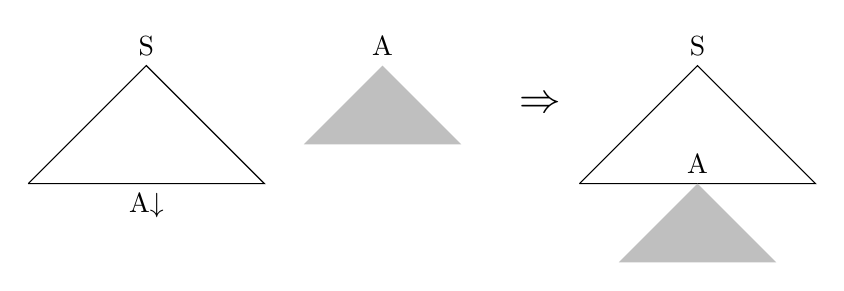
\begin{tikzpicture}[baseline]
  \draw (0,1)--(1.5,1)node[below]{A$\downarrow$}--(3,1)--(1.5,2.5)node[above]{S}--(0,1);
  % \node at (0.5,0.5) {\small$\alpha$};
  \filldraw[fill=lightgray,draw=none] (3.5,1.5)--(4.5,2.5)node[above]{A}--(5.5,1.5)--(3.5,1.5);
  % \node at (3.8,1) {\small$\beta$};
  \node[scale = 1.5] at (6.5,2) {$\Rightarrow$};
  \draw (7,1)--(8.5,1)node[below]{A}--(10,1)--(8.5,2.5)node[above]{S}--(7,1);
  \filldraw[fill=lightgray,draw=none] (8.5,1)node[anchor=south]{A}--(7.5,0)--(9.5,0)--(8.5,1);
  % \node at (8,-0.5) {\small$\gamma$};
\end{tikzpicture}
}
\z

\ea\label{ex:substitution-derivation}
\evnup{%
  \begin{forest}
    [S
      [NP$\downarrow$, name=target1, s sep = 10mm, calign=last
        [NP, no edge, name=np1 [N [Benjamin]]]
        [, phantom]
      ]
      [VP,baseline [V [loves]] 
        [NP$\downarrow$, name=target2, s sep = 10mm, calign=first
            [, phantom]
            [NP, no edge, name = np2 [N [Kasidy]]]
        ]
      ]
    ]
    \draw[->,thick,>=latex] (np1) to[out=90,in=270] (target1);
    \draw[->,thick,>=latex] (np2) to[out=90,in=270] (target2);
  \end{forest}
  %
  \hspace*{-1.5em}\scalebox{1.5}{$\Rightarrow$}\hspace*{1.5em}
  %
  \begin{forest}
    [S [NP [N [Benjamin]]] [VP,baseline [V [loves]] [NP [N [Kasidy]]] ]]
  \end{forest}
 }
\z

A tree rewriting grammar which makes use of substitution alone is called a
\fm{Tree Substitution Grammar} (TSG), and is at least weakly equivalent to a CFG
-- that is, such grammars describe the same set of string languages (weak
equivalence), although there are some tree languages which can be
described by a TSG for which an equivalent CFG does not exist (so strong
equivalence is not guaranteed).%
%
\footnote{Any CFG can easily be converted into a TSG by simply turning each
  phrase-structure rule into a tree rooted in the left-hand symbol with the
  right-hand symbols as daughters, as will be illustrated in the text. But to
  convert a TSG into a CFG, it may be necessary to relabel some nodes, since the
  dependency between a mother and its daughters may be tree-specific, and so not
  hold generally (for example, it might be the case that only trees anchored by
  transitive verbs have a VP dominating both a V and an NP node) -- so the CFG
  might have to have more non-terminal symbols than the TSG (e.g.
  VP$_\textnormal{trans}$ and VP$_\textnormal{intrans}$ instead of just VP).}
%
This is easy to see if we imagine converting a CFG into a TSG: all we do is
replace each phrase-structure rule with the equivalent tree which it describes
(cf. \citegenalt{mcca:68} conception of phrase-structure rules as node
admissibility conditions, i.e. descriptions of trees). For example, the CFG in
(\ref{ex:cfg}) corresponds to the TSG in (\ref{ex:tsg}):

\ea\label{ex:cfg}
\phraserule{S}{NP VP}\\
\phraserule{NP}{Miles}\\
\phraserule{VP}{V}\\
\phraserule{V}{sighs}
\z

\ea\label{ex:tsg}
\begin{forest}
  [S [NP$\downarrow$] [VP$\downarrow$]]
\end{forest}
\hspace*{2ex}
%
\begin{forest}
  [NP [Miles]]
\end{forest}
\hspace*{4ex}
%
\begin{forest}
  [VP [V$\downarrow$]]
\end{forest}
\hspace*{4ex}
%
\begin{forest}
  [V [sighs]]
\end{forest}
\hspace*{4ex}
%
\z

Although TSGs and CFGs are formally very close (at least weakly equivalent),
there is an important theoretical difference between them: TSGs have an
\fm{extended domain of locality} with respect to CFGs. Every rule in a CFG
describes a tree of depth 1, but trees in a TSG can be of arbitrarily large
size, which means that certain grammatical dependencies, like agreement or
extraction, can be described locally in a TSG (i.e. in a single elementary tree)
when they cannot be in a CFG (i.e. they cannot be described in a single rule).
For example, the TSG in (\ref{ex:tsg2}) is equivalent to that in (\ref{ex:tsg}),
except that now the verb and its subject are in the same elementary tree, and so
the agreement relationship between the two could be described locally.

\ea\label{ex:tsg2}
\begin{forest}
  [S [NP$\downarrow$] [VP [V [sighs]]]]
\end{forest}
\hspace*{2ex}
%
\begin{forest}
  [NP [Miles]]
\end{forest}
\hspace*{4ex}
%
\z

\noindent Many possibilities exist as to \emph{how} to describe such a
dependency -- for example, by using complex categories in the style of GPSG (on
which see \citealt{gkps}), or by using feature structures (on which see
Section~\ref{sec:TAG:contraints}); but the point is that however one chooses to
represent this relationship, it can be described locally in a TSG when it can
only be described indirectly in a CFG, e.g. by percolating features up from V to
VP, thus making them visible to the \mbox{S $\rightarrow$ NP VP} rule which
introduces the subject.


%%%%%%%%%%%%%%%%%%%%%%%%%%%%%%%%%%%%%%%%%%%%

\largerpage
\subsection{Adjunction}\label{sec:TAG:adjunction}

% Each instance of substitution requires a corresponding substitution site in
% the receiving tree. This makes it appropriate for combining a predicate with
% its arguments, since a predicate can be thought to explicitly specify how many
% arguments it requires.%
% %
% \footnote{Of course, this is rather a simplification: there are all manner of
% issues surrounding the classification of dependents \comment{SOME REFS!}}

If we add adjunction, a second type of combining operation, to a TSG, we obtain
a TAG. While substitution allows a tree to be inserted at a frontier node of
another tree, adjunction allows insertion at a \emph{non}-frontier node: the
adjoining tree expands the target node around itself. A tree which adjoins into
another tree, called an auxiliary tree, must therefore have at least one
frontier node with the same label as its root -- this is called the foot node.
The process of adjunction is represented schematically in
(\ref{ex:schematic-adjunction}):

\ea\label{ex:schematic-adjunction}\textbf{Adjunction} (after
\citealp[9]{abeille-rambow2000}) \evnup{%}
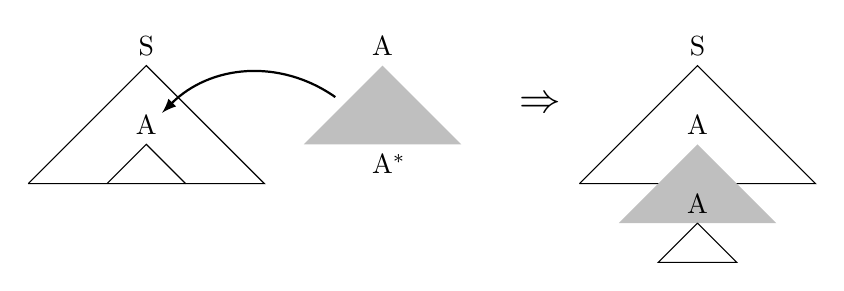
\begin{tikzpicture}
  % \draw[help lines] (0,-1) grid (10,3);
  \draw (0,1)--(1.5,1)--(3,1)--(1.5,2.5)node[above]{S}--(0,1);
  \draw (1,1)--(1.5,1.5)node[above]{A}--(2,1);
  % \node at (0.5,0.5) {\small$\alpha$};
  % \node at (0.5,0.5) {\fbox{$\alpha$}};
  \filldraw[fill=lightgray,draw=none] (3.5,1.5)--(4.5,2.5)node[above]{A}--(5.5,1.5)--(4.5,1.5)node[below]{A\footnode}--(3.5,1.5);
  % \node at (3.8,1) {\small$\beta$};
  % \node at (4,1) {\fbox{$\beta$}};
  \node[scale=1.5] at (6.5,2) {$\Rightarrow$};
  \draw (7,1)--(8.5,1)node[below]{A}--(10,1)--(8.5,2.5)node[above]{S}--(7,1);
  \filldraw[fill=lightgray,draw=none] (8.5,1.5)node[above]{A}--(7.5,0.5)--(9.5,0.5)--(8.5,1.5);
  \draw (8.5,0.5)node[above]{A}--(8,0)--(9,0)--(8.5,0.5);
  % \node at (8,-0.5) {\small$\gamma$};
  % \node at (8,-0.5) {\fbox{$\gamma$}};
  \draw [thick,->,>=latex] (3.9,2.1) to [out=145,in=45] (1.7,1.9);
\end{tikzpicture}
}
\z

Because of the requirement that the root and foot of an auxiliary tree have the
same label, such trees can be seen as factoring recursion out of the grammar.
Rather than having a cyclic path through the rewrite rules (as in a CFG), we
have a tree which directly encodes such a cycle (in
(\ref{ex:schematic-adjunction}), an A contained within an A), which can then be
added into a structure via adjunction. For this reason, such auxiliary trees are
used to model the recursive aspects of natural language syntax -- most notably
modification and sentential embedding.

Modifiers such as adjectives and adverbs, but also e.g. relative clauses, are
represented as auxiliary trees. For example, \textit{really} is a VP-adverb
which appears to the left of the VP it modifies, and so is represented by the
tree in (\ref{ex:really-tree}):


\largerpage[2]

\ea\label{ex:really-tree}
\begin{forest}
    [VP [AdvP [Adv [really]]] [VP\rlap{*}] ]
\end{forest}
\z\clearpage
%
To see this in use, consider the derivation for the sentence \textit{Benjamin
  really loves Kasidy}: after the substitutions shown above in
(\ref{ex:substitution-derivation}) to generate \textit{Benjamin loves Kassidy},
we can then adjoin the tree from (\ref{ex:really-tree}) at the VP node in the
clause, as in (\ref{ex:modifier-derivation}):

\ea\label{ex:modifier-derivation}
\evnup{%
\scalebox{0.85}{%
\begin{forest}
    [,phantom
        [S 
            [NP [N [Benjamin]]]
            [VP, baseline, name=vp [V [loves]] [NP [N [Kasidy]]]]
        ]
        [,phantom 
            [VP, name=adv [AdvP [Adv [really]]] [VP\footnode] ]
        ]
    ]
    \draw[thick,->,>=latex] (adv) to[out=130,in=45] (vp);
\end{forest}
%
\scalebox{1.5}{$\Rightarrow$}
%
\begin{forest}
    [S [NP [N [Benjamin]]] [VP,baseline [AdvP [Adv [really]]] [VP [V [loves]] [NP [N [Kasidy]]] ]]]
\end{forest}
}
}
\z
%
Of course, such a process can be repeated indefinitely many times, since there
is always still a tree-internal VP node available to be adjoined to, as in (\ref{ex:repeated-modifier-derivation}):

\eabox{\label{ex:repeated-modifier-derivation}
\evnup{%
\scalebox{0.75}{%
\begin{forest}
    [,phantom
        [S 
            [NP [N [Benjamin]]]
            [VP, baseline, name=vp 
                [AdvP [Adv [really]]]
                [VP [V [loves]] [NP [N [Kasidy]]]]
            ]
        ]
        [,phantom 
            [VP, name=adv [AdvP [Adv [really]]] [VP\footnode] ]
        ]
    ]
    \draw[thick,->,>=latex] (adv) to[out=130,in=45] (vp);
\end{forest}
%
\scalebox{1.5}{$\Rightarrow$}
%
\begin{forest}
    [S [NP [N [Benjamin]]] [VP,baseline [AdvP [Adv [really]]] [VP [AdvP [Adv [really]]] [VP [V [loves]] [NP [N [Kasidy]]] ]]]]
\end{forest}
}
}
}
%
This accounts for the iterability of modifiers like \textit{really}.

Another, perhaps more theoretically interesting, area of recursion in the
grammar is in the domain of subordination, i.e. sentential embedding. Verbs
which take sentential complements are represented as auxiliary trees, as in
(\ref{ex:likes-tree}), for example:

\ea\label{ex:likes-tree}
\begin{forest}
[S
    [NP$\downarrow$]
    [VP
        [V [thinks]]
        [S\footnode]
    ]
]
\end{forest}
\z
%
Notice that this means that sentential arguments are treated rather differently
from other arguments in TAG: while arguments are normally combined with their
governors by means of the former being substituted into the latter, sentential
arguments combine with their governors by means of the latter being adjoined
into the former -- this is shown in (\ref{ex:simple-sentential-embedding}):
\largerpage

\ea\label{ex:simple-sentential-embedding}
\scalebox{0.75}{
\attop{%
\begin{forest}
    [,phantom
        [,phantom
            [S,name=s2
                [NP [N [Benjamin]]]
                [VP
                    [V [loves]]
                    [NP [N [Kasidy]]]
                ]
            ]
        ]
        [S,name=s1
            [NP,baseline [N [Jake]]]
            [VP
                [V [thinks]]
                [S\footnode]
            ]
        ]
    ]
    \draw[thick,->,>=latex] (s1) to[out=120,in=45] (s2);
  \end{forest}%
%
\hspace*{1em}\scalebox{1.5}{$\Rightarrow$}\hspace*{1em}%\\
%
\begin{forest}
[S
    [NP [N [Jake]]]
    [VP
        [V, baseline [thinks]]
        [S
            [NP [N [Benjamin]]]
            [VP
                [V [loves]]
                [NP [N [Kasidy]]]
            ]
        ]
    ]
]
\end{forest}
}}
\z

% \newcommand{\tagdiagramscale}{0.7}
% \begin{figure}[htb]
% \centering
% % \scalebox{\tagdiagramscale}{%
% \resizebox{\textwidth}{!}{%
% \attop{%
% \begin{forest}
%     [,phantom
%         [,phantom
%             [S,name=s2
%                 [NP [N [Benjamin]]]
%                 [VP
%                     [V [loves]]
%                     [NP [N [Kasidy]]]
%                 ]
%             ]
%         ]
%         [S,name=s1
%             [NP,baseline [N [Jake]]]
%             [VP
%                 [V [thinks]]
%                 [S\footnode]
%             ]
%         ]
%     ]
%     \draw[thick,->,>=latex] (s1) to[out=120,in=45] (s2);
%   \end{forest}%
% %
% % \hspace*{1em}
% \scalebox{1.5}{$\Rightarrow$}%\\
% %
% \begin{forest}
% [S
%     [NP [N [Jake]]]
%     [VP, baseline
%         [V [thinks]]
%         [S
%             [NP [N [Benjamin]]]
%             [VP
%                 [V [loves]]
%                 [NP [N [Kasidy]]]
%             ]
%         ]
%     ]
% ]
% \end{forest}
% }}
% %}
% \caption{Sentential embedding via adjunction}
% \label{ex:simple-sentential-embedding}
% \end{figure}
%
For simple declarative sentences this is a rather unnecessary complication,
since the same effect could be achieved by making the foot node of the
sentential-embedding verb a substitution site instead. However, the factoring of
recursion into auxiliary trees interacts with another TAG principle -- the local
representation of syntactic dependencies. Owing to their extended domain of
locality, it is possible to represnt many kinds of syntactic dependencies
locally (i.e. in a single elementary structure) in TAG that would require some
additional mechanism in other frameworks. This principle extends to filler-gap
relations as well, such as that between a fronted focus phrase and its verbal
governor, as in (\ref{ex:fronting}):

\ea\label{ex:fronting}
\textit{Kassidy} Benjamin loves (whereas Kira he merely likes).
\z
%
The tree in (\ref{ex:love-extracted-tree}) represents the appropriate form of
the verb \textit{loves}, with its object extracted:%
%
\footnote{The use of a trace in object position here is not an essential part of
  the TAG analysis, though in practice it is common. One reason for this, as
  argued for by \citet{kroch:subjacency} and \citet{kroch:linguisticrelevance},
  is that empty elements allow for easier specification of some constraints on
  extraction in terms of the topology of trees, rather than necessitating
  additional mechanisms, like functional uncertainty and off-path constraints in
  LFG. A reviewer points out that traces are also useful in the metagrammar (see
  Section~\ref{sec:TAG:metagrammars} on this concept), since they allow tree
  fragments to be reused more easily.}

\ea\label{ex:love-extracted-tree}
\begin{forest}
[S\rlap{$'$}
    [NP$_i\downarrow$]
    [S
        [NP$\downarrow$]
        [VP
            [V [loves]]
            [NP [$t_i$]]
        ]
    ]
]
\end{forest}
\z
%
Through substitution alone, this can be used to derive
(\ref{ex:simple-extracted-tree}):

\ea\label{ex:simple-extracted-tree}
\begin{forest}
[S\rlap{$'$}
    [NP$_i$ [N [Kassidy]]]
    [S
        [NP [N [Benjamin]]]
        [VP
            [V [loves]]
            [NP [$t_i$]]
        ]
    ]
]
\end{forest}
\z
%
But of course the distance between the fronted phrase and the gap can span
multiple clauses, and can be arbitrarily large, as shown in (\ref{ex:ldd}):

\ea\label{ex:ldd}
\emph{Kassidy} [Jadzia knows [Jake thinks \dots\  [Benjamin loves]]].
\z
%
Since sentential embedding verbs are treated as auxiliary trees, this poses no
problem -- they are adjoined to the internal S node, and thus extend the
distance between the gap and the filler:

\ea\label{ex:ldd-derivation}
\evnup{%
\scalebox{0.7}{%
% \resizebox{\textwidth}{!}{%
% \attop{%
\vspace{-5em}
\hspace*{-2em}
\begin{forest}
[,phantom
    [S\rlap{$'$}
        [NP$_i$ [N [Kassidy]]]
        [S,name=s2
            [NP [N [Benjamin]]]
            [VP
                [V [loves]]
                [NP [$t_i$]]
            ]
        ]
    ]
    % [,phantom
        [S,name=s1
            [NP [N [Jake]]]
            [VP,baseline
                [V [thinks]]
                [S\footnode]
           ]
        ]
    % ]
]
\draw[thick,->,>=latex] (s1) to[out=120,in=45] (s2);
\end{forest}%
%
\hspace*{1em}\scalebox{1.5}{$\Rightarrow$}%\hspace*{1em}
%}
% \\[0.5em]
%
\begin{forest}
[S\rlap{$'$}
    [NP$_i$ [N, baseline [Kassidy]]]
    [S
        [NP [N [Jake]]]
        [VP
            [V [thinks]]
            [S,name=s2
                [NP [N [Benjamin]]]
                [VP
                    [V [loves]]
                    [NP [$t_i$]]
                ]
            ]
        ]
    ]
]
\end{forest}
}}
\z

% \begin{figure}[htb]
% \centering
% % \scalebox{\tagdiagramscale}{%
% \resizebox{\textwidth}{!}{%
% \attop{%
% % \evnup{%
% \begin{forest}
% [,phantom
%     [S\rlap{$'$}
%         [NP$_i$ [N [Kassidy]]]
%         [S,name=s2
%             [NP [N [Benjamin]]]
%             [VP
%                 [V [loves]]
%                 [NP [$t_i$]]
%             ]
%         ]
%     ]
%     % [,phantom
%         [S,name=s1
%             [NP [N [Jake]]]
%             [VP,baseline
%                 [V [thinks]]
%                 [S\footnode]
%            ]
%         ]
%     % ]
% ]
% \draw[thick,->,>=latex] (s1) to[out=120,in=45] (s2);
% \end{forest}
% %
% \hspace*{1em}\scalebox{1.5}{$\Rightarrow$}
% %}
% \\[0.5em]
% %
% \begin{forest}
% [S\rlap{$'$}
%     [NP$_i$ [N [Kassidy]]]
%     [S
%         [NP [N [Jake]]]
%         [VP
%             [V [thinks]]
%             [S,name=s2
%                 [NP [N [Benjamin]]]
%                 [VP
%                     [V [loves]]
%                     [NP [$t_i$]]
%                 ]
%             ]
%         ]
%     ]
% ]
% \end{forest}
% }%
% }
% \caption{Adjunction can produce long-distance dependencies}
% \label{ex:ldd-derivation}
% \end{figure}
%
What is more, this can clearly be repeated: other trees can be adjoined at the
topmost S node, further increasing the distance between the filler and the gap.
Thus, a potentially quite radically non-local dependency, between the fronted
expression and its governing verb, can be expressed locally in the grammar, in a
single elementary tree, because the operation of adjunction allows for the
distance between nodes in a tree to grow over the course of a derivation. This
same process can be applied to other kinds of filler-gap dependencies, such as
\textit{wh}-questions and relative clauses, though for ease of exposition I have
chosen not to illustrate these here (since for these we must also account for
things like subject-auxiliary inversion and \textit{do}-support).%
%
\footnote{The interested reader should consult the detailed analyses of these
  and other constructions in English provided by the XTAG project \citep{xtag}.}
%
The TAG approach is
in contrast to that of many other syntactic theories which instead derive or
infer the relation between filler and gap via some additional syntactic
mechanism, be that movement or, in the case of LFG, a functional uncertainty
path.
%In Section~\ref{sec:TAG:ldd-comparison}, we will compare the LFG and TAG
%approaches to long-distance dependencies in more detail.

%%%%%%%%%%%%%%%%%%%%%%%%%%%%%%%%%%%%%%%%%%%%

\subsection{Expressing constraints}\label{sec:TAG:contraints}

Adjunction of an auxiliary tree, which has a root and foot node with the same
label, captures the effects of recursion in other formalisms. However, once an
auxiliary tree has been adjoined in, there will be two nodes with the same label
where there was previously just one. This means that if we adjoin the same tree
again (e.g. as in (\ref{ex:repeated-modifier-derivation}), where we adjoin
\textit{really} twice), there are two distinct possible targets (and after that
adjunction there will be three, etc.). This has the potential to dramatically
complicate parsing, since there will be multiple distinct possible derivations
for the same tree (without there also being a genuine ambiguity of
interpretation), and so we would like a means of controlling where adjunction
takes place. TAG originally did this by using local constraints on adjunction
\citep[100ff.]{joshi1987}, annotations added to the nodes of elementary trees
indicating which auxiliary trees can be adjoined there. If the list of adjoiners
is empty, we have a \fm{null adjunction} (NA) constraint, which prohibits
adjunction at the node. If the list is non-empty, then we have a \fm{seletive
  adjunction} (SA) constraint, which limits the trees which can adjoin. There
are also \fm{obligatory adjunction} (OA) constraints, which are like SA
constraints except that one of the listed trees \emph{must} be adjoined at the
annotated node. In classic TAG, this is achieved simply by a diacritic
indicating that the constraint is an OA one rather than an SA one. We will see
below how this can be achieved in a less stipulative way by making use of
feature structures.

Using these constraints, we can avoid having multiple possible parses for
sentences by marking the foot node of auxiliary trees with an NA constraint (as
is done in the XTAG grammar of English, for example -- \citealp{xtag}). This
means we do not add an extra potential target for adjunction each time such a
tree is adjoined in, since only the root of the auxiliary tree is available for
further adjunction.

In addition to this practical motivation, adjunction constraints play a crucial
theoretical role: they are a vital part of what makes TAG mildly context
sensitive. Without adjunction constraints, the formalism is still more powerful
than a CFG, but there are several mildly context-sensitive languages which it
cannot express, such as the copy language $\{ww\ \vert\ w \in \Sigma^{*}\}$, or
the language $\{a^nb^nc^n\ \vert\ n \geq 0\}$, also called \textsc{count-3}
(\citealt[27, 58]{Kallmeyer2010}; we return to \textsc{count-3} in
Section~\ref{sec:TAG:generative-capacity}).

Let us now consider an example illustrating the linguistic utility of selective and obligatory adjunction constraints.
\citet[134--135]{vijayshanker1987} considers non-finite sentential complements
such as (\ref{ex:pro-clause}):

\ea John tried [PRO to leave].\label{ex:pro-clause}\z
%
Assuming the subordinate clause has the tree in (\ref{ex:pro-tree}), our
analysis needs to do two things: ensure that such clauses cannot appear on their
own as full sentences -- as illustrated in~(\ref{ex:bad-solo-pro}) -- and ensure that they can
be embedded only under verbs that select for infinitival forms --
as illustrated in~(\ref{ex:bad-embedded-pro}).

\ea\label{ex:pro-tree}
\begin{forest}
  [S
    [NP [PRO]]
    [VP [to leave, roof]]
  ]
\end{forest}
\z

\ea *To leave.\label{ex:bad-solo-pro}
\z

\ea\label{ex:bad-embedded-pro}
\ea John tried to leave.
\ex *John imagined to leave.
\z
\z
%
In other words, \emph{something} must be adjoined into the root node S (an OA
constraint), and that something must only be a sentential embedding verb that
selects for a non-finite complement clause (an SA constraint).

\hspace*{-5.3pt}Originally, these constraints were simply seen as listings of (permitted\slash
required) auxiliary trees, but this is not particularly linguistically
illuminating, and also difficult to maintain for a grammar writer. This is
remedied in later TAG work through the use of feature structures.
%
It is common to associate nodes with feature structures in CFG-based grammars
(e.g. in GPSG -- \citealt{gkps}) in order to represent grammatical features such
as case, number, tense, etc. Indeed, this is what LFG's \fstruc{}s do too
(although there multiple structures from different nodes are merged into one).
However, in a TAG, we cannot guarantee the integrity of each node in the tree:
through adjunction, it may be split up into two nodes, corresponding to the root
and foot nodes of an auxiliary tree. For this reason, in feature structure-based
TAG (FTAG: \citealp[ch.~5]{vijayshanker1987}; \citealp{vijayshanker-joshi1988}),
each node is associated with a \emph{pair} of feature structures, called the
\fm{top} and \fm{bottom} feature structures. The top features refer to the
relation of the node to its siblings and its ancestors, i.e. the view from above
the node in a tree. The bottom features refer to its relation to its
descendants, i.e. the view from below \citep[129]{vijayshanker1987}. Ultimately,
the top and bottom features of a node must unify, to give a single description
of the properties of that node. However, during the course of a derivation,
adjunction may split up the node so that it is now two nodes instead; in that
case, its top features will be unified with the top features of the root of the
auxiliary tree involved, and its bottom features will be unified with the bottom
features of the auxiliary tree's foot node. This is shown schematically in
(\ref{ex:ftag-adjunction}):

\ea\label{ex:ftag-adjunction}
\textbf{Adjunction in FTAG} (after \citealt[130]{vijayshanker1987})
\evnup{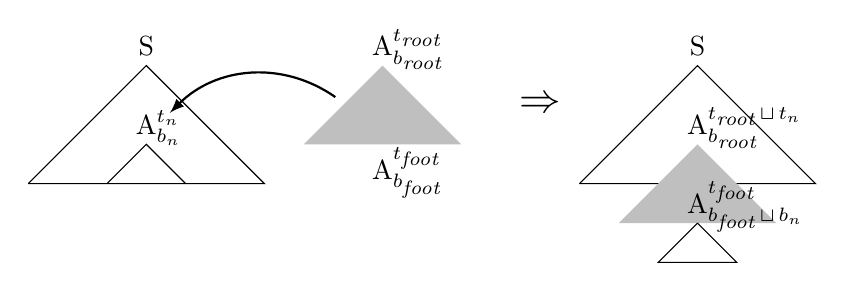
\begin{tikzpicture}
  % \draw[help lines] (0,0) grid (10,3);
  \draw (0,1)--(1.5,1)--(3,1)--(1.5,2.5)node[above]{S}--(0,1);
  \draw (1,1)--(1.5,1.5)node[above]{\smash{A\nodelabels{t_n}{b_n}}}--(2,1);
  % \node at (0.5,0.5) {\small$\alpha$};
  \filldraw[fill=lightgray,draw=none]
  (3.5,1.5)--(4.5,2.5)node[above]{\smash{A\nodelabels{t_\textit{\scriptsize
          root}}{b_\textit{\scriptsize root}}}}--(5.5,1.5)--(4.5,1.5)node[below=-2.5pt]{A\nodelabels{t_\textit{\scriptsize
          foot}}{b_\textit{\scriptsize foot}}}--(3.5,1.5);
  % \node at (3.8,1) {\small$\beta$};
  \node[scale=1.5] at (6.5,2) {$\Rightarrow$};
  \draw (7,1)--(10,1)--(8.5,2.5)node[above]{S}--(7,1);
  %
  \filldraw[fill=lightgray,draw=none] (8.5,1.5)node[above]{\smash{A\nodelabels{t_\textit{\scriptsize
          root}\, \sqcup\, t_n}{b_\textit{\scriptsize
          root}}}}--(7.5,0.5)--(9.5,0.5)--(8.5,1.5);
  %
  \draw (8.5,0.5)node[above]{\smash{A\nodelabels{t_\textit{\scriptsize
          foot}}{b_\textit{\scriptsize foot}\, \sqcup\, b_n }}}--(8,0)--(9,0)--(8.5,0.5);
  % \node at (8,-0.5) {\small$\gamma$};
  \draw [thick,->,>=latex] (3.9,2.1) to [out=145,in=45] (1.8,1.9);
\end{tikzpicture}}
\z
%
Substitution is simpler, since the root node of the substituted tree is simply
identified with the substitution site, and so both top and bottom feature
structures unify, as shown in (\ref{ftag:substitution}):%
%
\footnote{The diagram in (\ref{ftag:substitution}) follows
  \citegen{vijayshanker1987} original formulation, where substitution sites also
  contain bottom features. In much other work using FTAG, this is not the case,
  so $b_{n}$ in (\ref{ftag:substitution}) would be absent, and the final bottom
  features of A in the derived tree would simply be $b_{m}$ \citep[13]{xtag}.
  This is of course equivalent to (\ref{ftag:substitution}) with $b_{n}$
  instantiated as the empty feature structure.}
%

\ea\label{ftag:substitution}
\textbf{Substitution in FTAG}
\evnup{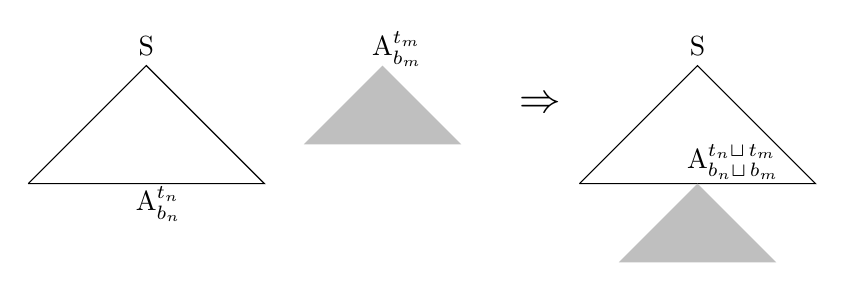
\begin{tikzpicture}[baseline]
  \draw (0,1)--(1.5,1)node[below=-2.5pt]{A\nodelabels{t_n}{b_n}}--(3,1)--(1.5,2.5)node[above]{S}--(0,1);
  % \node at (0.5,0.5) {\small$\alpha$};
  \filldraw[fill=lightgray,draw=none] (3.5,1.5)--(4.5,2.5)node[above]{\smash{A\nodelabels{t_m}{b_m}}}--(5.5,1.5)--(3.5,1.5);
  % \node at (3.8,1) {\small$\beta$};
  \node[scale = 1.5] at (6.5,2) {$\Rightarrow$};
  \draw (7,1)--(8.5,1)node[below]{A}--(10,1)--(8.5,2.5)node[above]{S}--(7,1);
  \filldraw[fill=lightgray,draw=none] (8.5,1)node[above=2pt]{\smash{A\nodelabels{t_n
        \sqcup\, t_m}{b_n \sqcup\, b_m}}}--(7.5,0)--(9.5,0)--(8.5,1);
  % \node at (8,-0.5) {\small$\gamma$};
\end{tikzpicture}
}
\z

These feature structures can be used to enforce various linguistic constraints.
For example, we can enforce subject agreement in initial trees for verbs by
specifying number and person features on the subject NP position.
%
% \ea\label{ex:agreement-tree-features}
%  \begin{forest}
%     [S
%       [NP\nodelabels{[\textsc{pers}\,3]}{$\avm{[x & y]$}}, name=target1, s sep = 10mm, calign=last
%         [NP, no edge, name=np1 [N [Miles]]]
%         [, phantom]
%       ]
%       [VP,baseline [V [yawns]]
%         ]
%       ]
%     \draw[->,thick,>=latex] (np1) to[out=90,in=270] (target1);
%   \end{forest}
%   %
% \scalebox{1.5}{$\Rightarrow$}\hspace*{1.5em}
%   %
%   \begin{forest}
%     [S [NP [N [Miles]]] [VP,baseline [V [yawns]] ]]
%   \end{forest}
% \z
%
More interestingly, we can use features to account for the constraints on
adjunction discussed above. Because the features associated with whatever tree
is adjoined at a node have to unify appropriately with its top and bottom
features, we can control which trees are compatible by giving them (mis)matching
features which make unification possible or not. What is more, we can give a
more principled account of obligatory adjunction constraints by making the top
and bottom features of a particular node incompatible with one another. This
means that unless adjunction takes place and the node is split up, unification
will be impossible, and the derivation will fail. Returning to our example from
above, (\ref{ex:pro-tree-features}) shows the tree from (\ref{ex:pro-tree}) with two added feature
annotations:

\ea\label{ex:pro-tree-features}
\begin{forest}
  [S\nodelabels%
  {[\textsc{tense}\,+]}{[\textsc{tense}\,-]}
  %{\avm{[tense & +]}}{\avm{[tense & -]}}
    [NP [PRO]]
    [VP [to leave, roof]]
  ]
\end{forest}
\z
%
Since these features are incompatible and cannot unify, we have achieved the
first of our goals, which is to ensure that this tree cannot appear on its own
-- i.e., to implement an OA constraint. Owing to the feature mismatch, this tree
is illicit unless something adjoins to the root node. To achieve the SA
constraint, we need to consider the elementary trees of verbs like
\textit{tried} and \textit{imagined}. In (\ref{ex:tried-tree}) and (\ref{ex:imagined-tree}) we present them with just the
relevant features added:

\ea\label{ex:tried-tree}
\begin{forest}
  [S\nodelabels{}{[\textsc{tense}\,+]}
  [NP$\downarrow$]
  [VP [V [tried]] [S\nodelabels{*[\textsc{tense}\,-]}{}]]
  ]
\end{forest}
\ex\label{ex:imagined-tree}
\begin{forest}
  [S\nodelabels{}{[\textsc{tense}\,+]}
  [NP$\downarrow$]
  [VP [V [imagined]] [S\nodelabels{*[\textsc{tense}\,+]}{}]]
  ]
\end{forest}
\z
%
The difference between the two verbs is that \textit{tried} selects for a
non-finite, untensed, complement clause, whereas \textit{imagined} selects for a
tensed one -- this is indicated by the top features on their foot nodes. If we
attempt to adjoin \textit{imagined} into the tree for the subordinate clause in
(\ref{ex:pro-tree-features}), then we end up with mismatching features on the
foot node, which means they cannot unify, and the tree remains illicit, as shown in (\ref{ex:imagined-tree-combined}):

\ea\label{ex:imagined-tree-combined}
\begin{forest}
  [S\nodelabels{[\textsc{tense}\,+]}{[\textsc{tense}\,+]}
  [NP$\downarrow$]
  [VP
    [V [imagined]]
    [S\nodelabels{[\textsc{tense}\,+]}{[\textsc{tense}\,-]}, name=s
    [NP [PRO]]
    [VP [to leave, roof]]
    ]
  ]
  ]
  \node [right = 3.6em of s.north east] (a){};
  \node [right = 3.6em of s.south east] (b){};
  \draw (s.south west) -- (s.north west) -- (a.center) -- (b.center) -- (s.south west);
\end{forest}
\z
%
If we adjoin the tree for \textit{tried}, however, then there is no mismatch,
and the derivation succeeds.

If we allow a fully-fledged unification-based feature system in FTAG, with
recursive feature structures of potentially unbounded size, then FTAG becomes
undecidable \citep[155f.]{vijayshanker1987}. This is a very bad result given the
emphasis that TAG places on tractable, polynomial parsing. For this reason, the
feature structures in FTAG are more restricted, and do not permit
recursion\slash re-entrancy, which makes them quite unlike LFG's \fstruc{}s.

% \begin{itemize}
%   \item Feature structure-based TAG (FTAG): associates elementary trees with
%         feature structures, to capture facts like agreement, tense, \GF s, etc.
%         \citep[ch.~5]{vijayshanker1987},\citep{vijayshanker-joshi1988}.
%   \item Nodes bear two feature structures (\textit{top} and \textit{bottom}
%         features), which must ultimately unify (this allows for adjunction
%         `splitting up' nodes).
%   \item Unlike LFG \struc{f}s, recursive/unbounded reentrancy is not permitted.
%   \item Each node is associated with a single (pair of) feature structure(s) (as
%         if $\phi$ was one-to-one). -- some of the purported advantages of FTAG
%         seem to stem from an assumption that unification-based theories always
%         associate a single feature structure with each node, e.g. the example of
%         agreement info having to be passed up from V to VP to be checked against
%         subject. This is not the case in LFG, right? We can state attributes of
%         (\^ SUBJ NUM) directly from verb. I guess what's happening is that
%         instead of passing attributes up, we are identifying the feature
%         structures. So \^ doesn't refer to a specific f-structure, because we
%         don't know what M(*) is yet. Does this matter??
% \end{itemize}


%%%%%%%%%%%%%%%%%%%%%%%%%%%%%%%%%%%%%%%%%%%%

\subsection{Derivation trees and dependencies}\label{sec:TAG:dependencies}

In a CFG as classically conceived, the familiar phrase-structure tree is in fact
a representation of the derivation, i.e. of the process by which the output,
namely the string, was produced. TAGs also have these \fm{derivation trees},
representing the way in which trees were combined during a derivation -- but, of
course, in a TAG, the output of the derivation is already a tree, called the
\fm{derived tree} to set it apart. The derived tree represents word order,
constituency, and category information, like LFG's \cstruc. So what linguistic
information does a TAG derivation tree encode? Since each elementary tree in a
(lexicalised) TAG corresponds to a lexical item, the derivation tree actually
represents relations between lexical items, and so has much in common with a
dependency grammar representation of the sort illustrated by Meaning-Text Theory
\citep{Melcuk1988}, the more contemporary Universal Dependencies project (UD:
\citealp{UD}), or, indeed, an LFG \fstruc\ (on the relationship between
dependency grammars and LFG, see also \citetv{chapters/Dependency}).

\newpage
A derivation tree for \textit{Benjamin really loves Kasidy}, the derivation for
which was shown in (\ref{ex:substitution-derivation}) and
(\ref{ex:modifier-derivation}), is given in (\ref{ex:derivation-tree}) \citep[cf.][74ff.]{joshi:tag-formal-hbk}:

\ea\label{ex:derivation-tree}
\begin{forest}
  [love
  [Benjamin, edge label={node[midway,above left,font=\scriptsize]{\textsc{1}}}]
  [Kasidy, edge label={node[pos=0.6,left,font=\scriptsize]{\textsc{2.2}}}]
  [really, edge label={node[midway,above right,font=\scriptsize]{\textsc{2}}}]
  ]
\end{forest}
\z
%
Here nodes are labelled with the lexeme corresponding to the elementary tree in
question. Whenever a tree is substituted or adjoined into another tree, it
becomes its daughter in the derivation tree. The derivation tree in
(\ref{ex:derivation-tree}) shows that three trees, corresponding to
\textit{Benjamin}, \textit{Kasidy}, and \textit{really}, were combined with the
tree for \textit{love}. Each edge is also labelled, standardly with a node
address which indicates where the tree was substituted or adjoined.%
%
\footnote{These are so-called \fm{Gorn addresses} \citep{Gorn:67}. The root has
  the address $0$ (or sometimes $\epsilon$, i.e. the empty string), the $k$th
  child of the root (reading left-to-right) has the address $k$, and for all
  other nodes, the $q$th child of a node with address $p$ has the address $p.q$
  \citep[75]{joshi:tag-formal-hbk}.}
%
However, we can equally well use different labels, such as assigning grammatical
function names to argument positions and then treating other positions as \ADJ
\citep[cf.][175]{rambow:dependency}. This would give us the derivation
tree in (\ref{ex:derivation-tree-gf}) instead of (\ref{ex:derivation-tree}), making the parallel with dependency
structures quite explicit:

\ea\label{ex:derivation-tree-gf}
\begin{forest}
  [love
  [Benjamin, edge label={node[midway,above left,font=\scriptsize]{\textsc{subj}}}]
  [Kasidy, edge label={node[pos=0.6,left,font=\scriptsize]{\textsc{obj}}}]
  [really, edge label={node[midway,above right,font=\scriptsize]{\textsc{adj}}}]
  ]
\end{forest}
\z
%
\citet{rambow:dependency} discuss the relationship between TAG and dependency
grammars in more detail.

Unfortunately, the TAG treatment of sentential embedding somewhat undermines the
neat parallel between derivation trees and dependency structures
\citep{rambow:d-tree,rambow-etal2001}. Recall that arguments are normally
substituted into their governors, but that clausal complements have their
governors adjoined into them. This reverses the normal dependency relations, and
means that ``(standard) LTAG derivation trees do \emph{not} provide a direct
representation of the dependencies between the words of the sentence, i.e., of
the predicate-argument and modification structure'' \citep[117, emphasis in
original]{rambow-etal2001}. To see why this is so, consider the derivation tree
for (\ref{ex:simple-sentential-embedding}), \textit{Jake thinks Benjamin loves
  Kasidy}:

\ea
\begin{forest}
  [love
  [Benjamin]
  [Kasidy]
  [think [Jake]]
  ]
\end{forest}
\z
%
In (\ref{ex:TAG:thinkJake}) \textit{think} is a dependent of \textit{love}, because the \textit{think}
tree is adjoined into the \textit{love} tree, when of course in any real
dependency grammar the relation would be reversed:

\ea\label{ex:TAG:thinkJake}
\begin{forest}
  [think
  [Jake]
  [love
  [Benjamin]
  [Kasidy]
  ]
  ]
\end{forest}
\z

There are technical means of handling this unhappy result \citep[see
e.g.][]{joshi:semantics-published,Kallmeyer:Kuhlmann:12}, but it nevertheless
makes the parallel with dependency structures rather less direct. All the same,
we might be tempted to see the division of labour between derived trees and
derivation trees in TAG as analogous to that between \cstruc{} and \fstruc{} in
LFG, where the former represents constituency, word order, and category
information, and the latter encodes a sentence's dependency structure. This is
certainly true to a point, but the parallel is imperfect, because \fstruc{} also
represents other information beyond the dependency structure of a sentence --
syntatic features like person, number, tense, aspect, etc., which in TAG are
encoded in the feature structures associated with each node instead. Still, one
thing that derivation trees and \fstruc{}s have in common is that they are both
seen as the appropriate level of representation to serve as input to the
semantic component of the grammar.

%%%%%%%%%%%%%%%%%%%%%%%%%%%%%%%%%%%%%%%%%%%%

\subsection{Semantics}\label{sec:TAG:semantics}

There have been a variety of different proposals for interfacing TAG with a
semantic theory, and space precludes a full presentation here. Nonetheless, this section gives a (superficial) overview of the relevant literature, so that the interested reader can investigate
further.

An early proposal for doing semantics with TAG makes use of \fm{Synchronous TAG}
(STAG: \citealp{shieber-schabes1990}). In STAG, elementary trees from one
grammar are paired with those from another, and links are established between
individual nodes in those trees. Then, when adjunction or substitution applies
in one grammar, it must also take place in the other, at the linked node, and
using the equivalent, paired tree. By pairing a TAG grammar with a tree-based
semantic representation, we can therefore implement a ``rule-to-rule'' approach
to semantic derivation (to use \citegenalt{bach:extension} terminology).%
%
\footnote{Alternatively, by pairing two TAG grammars from different languages,
  we can implement a machine translation system -- see
  \citet{abeille:translation}.}
%
Nothing requires the paired trees to be isomorphic, so on the syntactic side it
is the structure of the derivation tree, not the derived tree, which determines
the meaning. Although this approach has largely fallen out of favour in TAG
circles, see \citet{nesson:stag,Nesson:Shieber:07,Nesson:Shieber:08} for a
modern revival.

Another approach which uses the derivation tree as the basis for semantic
interpretation is that of \citet{joshi:semantics-published}. Here elementary
trees are associated with triples of semantic expressions, the first of which
specifies the main variable of the predication, the second of which gives the
predicate with its arguments, and the third of which specifies which argument
variables are associated with which nodes in the tree. When a tree is
substituted into another tree, its main variable is identified with the
corresponding argument variable in the target tree's semantics (special
consideration has to be made for adjunction, as discussed above: the order of
dominance in the derivation tree will be different for sentential vs.
non-sentential complements -- see \citealt[152f.]{joshi:semantics-published}).
Since this makes use of a unification-based semantics, the order of combination
of the elementary trees is irrelevant, and the derivation tree thus offers an
appropriate level of representation, since it abstracts away from order, and
simply says how and where trees were combined. This unification-based approach
has been developed more recently by Laura Kallmeyer and colleagues, introducing
a new focus on underspefication
\citep{gardent:semantics-ftag,kallmeyer:factoring,kallmeyer:unification,kallmeyer:scope}.
This has also been integrated with Frame Semantics
\citep{kallmeyer:frame-semantics}.

In LFG, the \textit{de facto} standard approach to the syntax-semantics interface
is \fm{Glue Semantics} (\citetv{chapters/Glue}). Observing that, for example, the
operation of function application as used in natural language semantics is order
insensitive, and that quantifier scope ambiguities show that semantic
interpretation does not (always) respect the constituent structure of a sentence
\citep[see][ch.~5]{Asudeh12}, Glue rejects \cstruc{} as the appropriate level of
input to semantics, and uses (a projection of) \fstruc{} instead (where order is
irrelevant and many \cstruc{} hierarchies are collapsed). Thus, as in TAG, it is
the dependency structure, not the phrasal structure, which is taken as relevant
for semantic interpretation.
Interestingly, however, one of the only examples of TAG theorists criticising
the derivation-tree-based approach to semantic interpretation is when Glue
Semantics has been combined with TAG \citep{frank:gluetag}.
\citeauthor{frank:gluetag} argue that the derivation tree is not
suitable as the input to semantic interpretation,  mostly on the basis that, as discussed above,
it provides the wrong dependency structure, and they instead make use of
the derived tree in their Glue-based framework.

%%%%%%%%%%%%%%%%%%%%%%%%%%%%%%%%%%%%%%%%%%%%

\subsection{The big picture}\label{sec:TAG:tag-summary}

Linguistic theories based on TAG have two key properties
\citep[95f.]{joshi:tag-formal-hbk}:
% , both of which set them apart from those based on LFG and many other frameworks:

\begin{enumerate}
  \item \textsc{Extended domain of locality}: Since TAG elementary trees
        encompass the whole extended projection of a lexical item, dependencies
        which in a simple CFG-based grammar would be spread across multiple
        rules, e.g. agreement, can be expressed ``locally'' in a TAG (i.e. in
        the same elementary structure). This is what enables a TAG to lexicalise
        a CFG (see Section~\ref{sec:TAG:lexicalisation}).
        % LFG gains some of this extended domain of locality via
        % f-structure, so that e.g. agreement can be encoded locally in the
        % agreement controller's lexical entry \citepv[see][]{chapter/Agreement},
        % but this does not extend to c-structure phenomena
  \item \textsc{Factoring recursion from the domain of dependencies}: Relatedly,
        the elementary trees are the structures over which the vast majority of
        dependencies are stated, and that includes filler-gap relations. Such
        dependencies are therefore local in nature, but can become long distance
        via the adjunction operation. Recursion is thereby factored out of the
        domain over which these dependencies are initially stated.
\end{enumerate}
%
This approach is summed up by \citet[2]{bangalore:introduction} in the slogan
``complicate locally, simplify globally''. That is, local, elementary
representations are where almost all linguistic constraints are stated, meaning
that they can become quite complex, but the payoff is that the composition of
elementary trees can be achieved by just two, very general, operations:
substitution and adjunction. This also means that cross-linguistic variation is
entirely a matter of what elementary trees a grammar contains, a position very
much in keeping what \citet[353]{baker2008macroparameter} calls the
\fm{Borer-Chomsky Conjecture}, after \citegen{borer:parametric} proposal and
\citegen{chomsky1995the-minimalist} later adoption of it, whereby parametric
variation is restricted to the lexicon.

How does this compare with LFG? The second property certainly divides the
frameworks: LFG grammars include recursive c-structure rules, and filler-gap
dependencies are expressed syntactically, not lexically. This means, moreover,
that the lexicon is not the only source of complexity in LFG grammars; many
constructions are analysed as instantiating complex annotated phrase structure
rules (see e.g. the analysis of long-distance dependencies in
\citealt[ch.~17]{DLM:LFG}). There is more overlap between the two frameworks
when it comes to the first property. Via the parallel projection architecture
(\citetv[see][sec.~5]{chapters/Intro}), LFG does obtain an extended domain of
locality: for example, agreement can be encoded locally in the agreement
controller's lexical entry via the use of paths through \fstruc\
(\citetv[see][]{chapters/Agreement}).
% And this does indeed lead in many cases to the lexicon being the major locus of complexity in the grammar. Not exclusively, however: constructions which are encoded by particular phrasal configurations, such as relative clauses, are still encoded in the phrase-structure grammar, sometimes using rules with quite complex and bespoke annotations (see e.g. the rule for relative clauses given in LFG grammars treat many phenomena as represented through sometimes quite complex annotated phrase structure rules, e.g. the analysis of relative clauses given in \citet{dalrymple01}
However, since \cstruc\ is generated by a CFG, any non-local dependencies
between \cstruc\ nodes (i.e. those spanning more than one ``generation'' in the
tree) can only be expressed indirectly via other levels of representation. That
is, we have no extended domain of locality at \cstruc\ \textit{per se}, only
parasitically via other levels.
% ADD REFERENCE TO MY JLM PAPER HERE LATER?
To the extent that phrasal constructions larger than a tree of depth 1 are
objects we want to be able to represent in the grammar, this is a shortcoming.
We return to this point in Section~\ref{sec:TAG:implications}.

\fm{Construction Grammar} (CxG:
\citealt{FillmoreKayOConnor1988,goldberg1995constructions,Goldberg2006,KayFillmore1999,BoasSag2012,HoffmannTrousdale2013},
\textit{i.a.}) of course considers such objects as basic to linguistic
theorising, and for this reason it has been argued that TAG is a natural means
of formalising CxG \citep{lichte:tag-cxg}. For example, among the properties of
constructions listed by \citet[501]{FillmoreKayOConnor1988}, one is that they
``need not be limited to a mother and her daughters, but may span wider ranges
of the sentential tree'' -- precisely the enlarged definition of locality which
a TAG provides, and which LFG denies (at least directly). TAG has a natural
means of representing both ``formal'' and ``substantive'' idioms, to use
\citegen{FillmoreKayOConnor1988} classification: formal idioms can be
included in the set of trees associated with each lexical item of the
appropriate class \citep[208f.]{lichte:tag-cxg}, and substantive idioms can be
represented as elementary trees in their own right \citep{abeille1995}. While
LFG can quite well represent formal idioms at the more schematic end of the
scale \citep[see e.g.][]{asudeh2013constructions}, it struggles with substantive
idioms, precisely because it lacks an extended domain of locality at \cstruc\
\citep[sec.~4]{findlay:lfg-as-cxg}.
%Given the increasing prominence of Construction Grammar ...

%%%%%%%%%%%%%%%%%%%%%%%%%%%%%%%%%%%%%%%%%%%%%%%%%%%%%%%%%%%%%%%%%%%%%%%%%%%%%%%%%%%%%%%%

\section{Generative capacity}\label{sec:TAG:generative-capacity}

TAG was designed specifically as a formalism with only mildly context-sensitive
power (in the technical sense of \citealt{joshi1985}). This means there are
languages out of the reach of context-free grammars that TAGs can describe, but
also that there are languages properly considered context sensitive which TAG
cannot. Such a constrained expansion into the context-sensitive space enables
parsing algorithms for TAG to preserve the computationally appealing property of
a polynomial run time.

As a simple demonstration of the increased generative capacity of a TAG when
compared to a CFG, consider the artificial formal language
$\{a^nb^nc^n\ \vert\ n \geq 0\}$, also known as \textsc{count-3} -- that is, the
language which contains all strings consisting of some number of $a$s followed
by the same number of $b$s, then the same number of $c$s.
\citet[497]{partee-etal1990} demonstrate through application of the pumping
lemma for context-free languages that \textsc{count-3} is not context free. By
contrast, there is a quite straightforward TAG grammar for \textsc{count-3},
shown in (\ref{ex:count-3-tag}):%
%
\footnote{Recall that a node annotated with ``NA'' bears a null adjunction
  constraint -- see Section~\ref{sec:TAG:contraints}. As mentioned above, without
  adjunction constraints, TAG becomes less expressive, and cannot describe
  \textsc{count-3}: see \citet[222]{Kallmeyer2010} for a proof.}
%

\ea\label{ex:count-3-tag}
\setlength{\tabcolsep}{20pt}
\begin{tabular}[t]{lll}
    \begin{forest}
      [S [$\epsilon$] ]%{\draw (.west) node[left] {$\alpha_{1}$};}
    \end{forest}
  % &
  %   \begin{forest}
  %     [S\nanode
  %       [a]
  %       [S
  %         [b]
  %         [c]
  %       ]
  %     ]%{\draw (.west) node[left] {$\alpha_{2}$};}
  %   \end{forest}
  &
    \begin{forest}
      [S\nanode
        [a]
        [S
          [b]
          [S\nafootnode]
          [c]
        ]
      ]%{\draw (.west) node[left] {$\beta_{1}$};}
    \end{forest}
\end{tabular}
\z

So, we can see that TAGs are more powerful than CFGs. They are not, however,
very much more powerful. There are many kinds of language which they cannot
describe, including those which it has been shown can be described by similarly
modest extensions to context-free grammars. One example of this is the language
MIX \citep{bach1981}, mentioned in footnote~\ref{fn:mix}, which consists of all
permutations of each string in the set $\{a^n b^n c^n\ \vert\ n \geq 0\}$, i.e.
any number of $a$s, $b$s, and $c$s, in any order, provided there is the same
number of each. \citeauthor{salvati2015} (\citeyear{salvati2015} -- originally
circulated as a technical report in 2011) showed that MIX is in the class of
multiple context-free languages, where a multiple context-free grammar (MCFG) is
itself a mildly context-sensitive grammar formalism, for which the parsing
problem is also decidable in polynomial time. However, MIX is \emph{not} a
tree-adjoining language, as conjectured by \citet{joshi-etal1991} and proved by
\citet{kanazawa-salvati2012}: so there are languages which are only slightly
within the context-sensitive space and which are still not describable by a TAG.
More generally, although \textsc{count-3} and \textsc{count-4} (i.e.
$\{a^nb^nc^n d^n\ \vert\ n \geq 0\}$) are tree-adjoining languages,
\textsc{count-5} is not \citep[223f.]{joshi1985}.

The carefully constrained computational complexity of TAG is in marked contrast
to the situation in LFG (although see below for attempts to constrain the power
of the LFG formalism). Whereas the class of tree-adjoining languages is
equivalent to that of the mildly context-sensitive languages (or, perhaps, the
slightly non-context-free languages: see fn.~\ref{fn:mix}), the languages
described by LFGs are equivalent to the class of recursively enumerable
languages \citep{nakanishi-etal1992}. This has the expected deleterious effect
on computational complexity: the parsing problem for LFGs is
$\mathsf{NP}$-complete \citep{Berwick1982}, and so, in the worst case scenario,
computationally intractable (assuming $\mathsf{P} \neq \mathsf{NP}$).

There have been attempts to remedy this situation, however. While the LFG
formalism as a whole may be computationally very complex, some of the properties
responsible for this are not relevant for the description of natural languages
-- this opens the possibility that the formalism could be constrained to allow
tractable parsing (i.e. in polynomial time) while still preserving its
usefulness as a tool for describing natural languages. \citet{SekiEtAl1993}
propose one such restriction, which limits the kinds of functional annotations
permitted on \cstruc\ nodes, and the number of nodes which can correspond to a
single \fstruc. This successfully buys tractability for the resulting formalism,
but at a heavy theoretical cost: many staple aspects of LFG analyses are no
longer available, including the very common \mbox{$\UP = \DOWN$} head-sharing
annotation, or functional control equations like
\mbox{$(\UP\ \XCOMP\ \SUBJ) = (\UP\ \SUBJ)$}. More recently, \citet{wed:kap:20}
have addressed this limitation, describing a more expressive but still tractable
version of the LFG formalism, which is provably equivalent to a Linear
Context-Free Rewriting System (LCFRS), and therefore in the mildly
context-sensitive space. (See also \citetv{chapters/Computational} and
references therein for discussion of the formal and computational properties of
LFG.) This approach only covers the original LFG formalism of
\citet{kaplanbresnan82}, however, and it remains to be seen whether certain
extensions to this basic formalism, such as functional uncertainty
\citep{kaplan-etal1987,kaplzaen89}, can be accommodated as straightforwardly in
this new approach.

One point worth noting is that even in the absence of a tractable version of
LFG, this contrast between TAG and LFG should not automatically be viewed as a
failing on the part of the latter. In fact, it reflects a rather deep
meta-theoretical question: do we want the formalism \emph{itself} to say
something interesting about the class of natural languages? The view embodied by
TAG is that we should be interested in ``finding a grammar
formalism that, by itself, gives already a close characterization of the class
of natural languages'' \citep[7]{Kallmeyer2010}.%
%
\footnote{This view is also shared by Combinatory Categorial Grammar (CCG: \citealt{steedman2000ccg}) and Multiple Context Free Grammars (MCFGs: \citealt{SekiEtAl1991}), among others.}
%
By contrast, the view embodied
by LFG is that ``it is the theory that imposes the
constraints, not the language in which the theory is expressed''
\citep[9]{poll:97:nature}.%
%
\footnote{This view is also shared by Head-Driven Phrase Structure Grammar (HPSG: \citealt{pollard1994head-driven}) and Minimalism \citep{chomsky1995the-minimalist}, among others.}
%
In theoretical terms, at least, it does not seem
obvious that one approach is \emph{better} than the other -- they are merely
different perspectives on the problem.%
%
\footnote{Of course, from a more practical point of view, it matters very much
  whether a formalism is tractable if it is to be used in some natural language
  processing task. However, there is already a very successful computational
  implementation of LFG in the form of the Xerox Linguistic Environment (XLE:
  \citealp{kaplannewman97}; \citealp{xledoc}), which employs various ``packed
  computation'' \citep{lev:packed-computation} heuristics to ensure efficient
  parsing \citep{maxwellkaplan89,maxwellkaplan93,maxwellkaplan96}. So whatever
  limitations may exist in principle, they do not necessarily apply in
  practice.}
%

%%%%%%%%%%%%%%%%%%%%%%%%%%%%%%%%%%%%%%%%%%%%%%%%%%%%%%%%%%%%%%%%%%%%%%%%%%%%%%%%%%%%%%%%

\section{Lexicalisation}\label{sec:TAG:lexicalisation}

I mentioned at the start of Section~\ref{sec:TAG:intro-to-tag} that linguistic
applications of TAG assume that the grammar is ``lexicalised''.
\citet[7]{abeille-rambow2000} give the following definition of this term
(emphasis in original):

\begin{quote}
  We will call a grammar \emph{lexicalised} if every elementary structure is
  associated with exactly one lexical item (which can consist of several words),
  and if every lexical item of the language is associated with a finite set of
  elementary structures in the grammar.
\end{quote}
% %
In contrast to (L)TAG, LFG grammars are not in general lexicalised, which is
perhaps somewhat surprising given what the ``L'' in ``LFG'' stands for. Although
there is a focus in LFG on the lexicon as a richly structured respository of
grammatical information, there is no requirement that this information
\emph{cannot} be expressed through non-lexical means. This section begins by
sketching the potential for lexicalising CFG-based formalisms, like LFG, and
then explores what the potential advantages of lexicalised grammars are.

In general, CFGs are not lexicalised. For example, the toy grammar in
(\ref{ex:cfg}), repeated below, is not lexicalised, since the first and third
rules are not associated with any lexical item -- they consist purely of
non-terminals.

\begin{exe}
  \exi{(\ref{ex:cfg})}
  \phraserule{S}{NP VP}\\
  \phraserule{NP}{Miles}\\
  \phraserule{VP}{V}\\
  \phraserule{V}{sighs}
\end{exe}
%
Since LFG is based on a CFG, via \cstruc, LFG grammars standardly make use of
many non-lexicalised rules like these, which means that LFG grammars are
generally not lexicalised.

It is possible to convert a non-lexicalised grammar into a lexicalised one, but
this can require a change to the formalism used. We can speak of one grammar
(weakly or strongly) \fm{lexicalising} another if the former is (weakly or
strongly) equivalent to the latter, except that the former is lexicalised
whereas the latter is not.%
%
\footnote{Two (classes of) grammars are weakly equivalent if they describe the
  same (sets of) string languages (though the corresponding (sets of) tree
  languages may differ). They are strongly equivalent if they also describe the
  same (sets of) tree languages.}
%
For example, the Tree Substitution Grammar shown above in (\ref{ex:tsg2}), and
repeated below, \fm{strongly lexicalises} the grammar in (\ref{ex:cfg}), since
each elementary object in (\ref{ex:tsg2}) is associated with a lexical item, and
the grammar describes the same string and tree language as (\ref{ex:cfg}).

\begin{exe}
  \exi{(\ref{ex:tsg2})}
\begin{forest}
  [S [NP$\downarrow$] [VP [V [sighs]]]]
\end{forest}
\hspace*{2ex}
%
\begin{forest}
  [NP [Miles]]
\end{forest}
\hspace*{4ex}
%
\end{exe}

Sometimes it is possible to use a CFG to strongly lexicalise another CFG, but it
turns out that this cannot be guaranteed in principle. For, although there is a
way of converting any CFG into so-called \fm{Greibach normal form}
\citep{greibach1965}, where the right-hand side of each rule begins with a
terminal symbol -- thereby lexicalising the grammar -- such grammars do not in
general generate the same set of trees as the grammars they normalise, since
they will include different (and many more) rules. That is, converting a CFG
into Greibach normal form only weakly lexicalises it. The extended domain of
locality of a TSG\slash TAG allows us to avoid this problem, however, and makes
tree grammars like this ``naturally'' lexicalised \citep[579]{schabes-etal1988}.
In fact, to strongly lexicalise an arbitrary CFG, we require a TAG, not simply a
TSG (see \citealt[22f.]{Kallmeyer2010} for a proof). And although a TSG may be
sufficient to lexicalise many linguistically relevant CFGs, it places
syntactically undesirable restrictions on the resulting grammar, and so a TAG is
preferable here too (\citealp[579]{schabes-etal1988};
\citealt[ch.~1]{schabes:phdthesis}). But why should we care whether a grammar is
lexicalised or not?

One early advantage touted for lexicalised grammars was based on parsing. In a
lexicalised grammar, a given sentence can contain at most as many elementary
structures as there are words in the sentence. Since each lexical item is
associated with a finite number of elementary structures, this also means that
the number of analyses for the sentence is finite, thus guaranteeing that the
recognition problem is decidable \citep[581f.]{schabes-etal1988}. As
\citet[21; emphasis in original]{Kallmeyer2010} puts it, ``[l]exicalized
grammars are \emph{finitely ambiguous}, i.e., no sequence of finite length can
be analyzed in an infinite number of ways''. However, in practice, the dangers
of non-terminating parses are virtually non-existent in sensibly-written
natural-language grammars, and so this advantage is not so great as it may
seem.%
%
\footnote{My thanks to Adam Przepi\'{o}rkowski and Timm Lichte for discussion of
  this point.}
%

A related claim is that lexicalised grammars assist parsing because ``parsing
need consider only those trees of the grammar that are associated with the
lexical symbols in the input string'' \citep[79f.]{eisner:parsing}, rather
than searching the whole grammar, and so the specific words used in a sentence
``help to restrict the search space during parsing'' \citep[20]{Kallmeyer2010}.
Once again, however, this argument carries less practical weight than it might
seem, since parsing times for TAG grammars are actually rather slow: the best
parsing algorithms for TAGs have a time complexity of $\mathcal{O}(n^6)$, as
opposed to $\mathcal{O}(n^3)$ in the case of CFGs, for example
\citep[ch.~5]{Kallmeyer2010}.%
%
\footnote{Although this is true of TAGs in general, if our only concern is
  lexicalising an existing CFG-based grammar, then we could likely devise a
  parser specialised for TAG grammars that lexicalise CFGs which would have a
  complexity below $\mathcal{O}(n^{6})$. My thanks to a reviewer for this
  observation.}
%

There are, however, more theoretical reasons to be interested in lexicalised
grammars. Firstly, it is by virtue of lexicalisation that the derivation tree of
a sentence corresponds to its dependency structure \citep[4ff.]{Kuhlmann2010},
as discussed in Section~\ref{sec:TAG:dependencies}. Because each elementary object
in a lexicalised grammar corresponds to a lexical item, by tracking the
combination of those objects we are in fact tracking the combination of lexical
items. Especially given the recent interest in dependency grammars prompted by
the Universal Dependencies project \citep{UD}, it is clearly advantageous if our
formalism has a transparent connection to dependency structures (see also
\citetv{chapters/Dependency} on the relationship between LFG and dependency
grammars).

Secondly, a lexicalised grammar fits very well with a lexicalist view of
syntactic theory. Since the 1970s (at least since the publication of
\citealt{chomsky1970remarks}), there has been a trend in linguistic theory
towards giving lexical analyses of many phenomena which were previously treated
as purely syntactic.
% (see e.g. \citealp{halle:prolegomena,jackendoff1975morphological} for some
% early theories of the lexicon along these lines).
Indeed, driven by this trend, a plethora of linguistic frameworks have emerged
which very deliberately place the lexicon front and centre, treating it as a
``richly structured'' object, and assuming ``an articulated theory of complex
lexical structure'' \citep[3]{dalrymple01} -- this includes LFG, as well as (to
a greater or lesser extent) Generalized Phrase Structure Grammar (GPSG:
\citealp{gkps}), Head-Driven Phrase Structure Grammar (HPSG:
\citealp{pollard1994head-driven}, \citealt{mullerwechsler14}), Combinatory Categorial Grammar (CCG:
\citealp{steedman2000ccg}), Minimalism \citep{chomsky1995the-minimalist}, and others. %
%
Such a focus on the richness of the lexicon is in stark contrast to the
historically more prominent view of it as a mere ``collection of the lawless'',
to use \citegen[4]{disciullo:word} term, where it is simply a repository of
exceptions, ``incredibly boring by its very nature'', about which ``there
neither can nor should be a theory'' (\textit{ibid.}: 3f.). Given that a
lexicalist syntactic theory assumes a richly detailed lexicon, in its most
parsimonious form this is \emph{all} it would require, the syntactic component
being encoded in the lexical entries themselves. In fact, this is just what
lexicalisation provides: in TAG, for example, aside from the basic operations of
adjunction and substitution, any other grammatical constraints are described in
the elementary trees of lexical items; that is, in the lexicon. In a lexicalised
grammar, the lexicon essentially \emph{is} the grammar.%
%
\footnote{Note that it is possible to collapse the lexicon\slash grammar
  distinction without also collapsing the word\slash phrase (or, equivalently,
  morphology\slash syntax) distinction: the processes which build word forms,
  i.e. the leaf nodes of elementary trees in TAG, need not be the same as those
  which build derived trees in the syntax. Thus, the formal language theory
  objections to Construction Grammar presented by
  \citet[4f.]{asudeh2013constructions} are only objections to the most radical
  version of the theory, and need not be taken as objections to constructional
  approaches generally.}
%
This means that every language shares the same computational component, and the
only differences between languages are in the lexicon (cf. the Borer-Chomsky
Conjecture, mentioned above). This is unlike LFG, for example, where languages
differ both in their lexica and in the set of \cstruc\ rules they employ.

%%%%%%%%%%%%%%%%%%%%%%%%%%%%%%%%%%%%%%%%%%%%%%%%%%%%%%%%%%%%%%%%%%%%%%%%%%%%%%%%%%%%%%%%%

\section{Factoring out redundancies}
\label{sec:TAG:metagrammars}


Natural language grammars involve a large amount of redundancy: for example, the
TAG elementary trees for \textit{loves} and \textit{thinks} shown in
Table~\ref{tab:elementary-trees} are identical except for their lexical anchors
and for the fact that \textit{loves} takes an NP complement where
\textit{thinks} takes an S complement. Similarly, all proper nouns will have
elementary trees like \textit{Benjamin}, and all VP adverbs will have elementary
trees like \textit{really}, except they may follow rather than precede the VP
they modify (i.e. the order of the foot node VP* and the AdvP node may be
reversed). There is less redundancy when it comes to trees in an LFG grammar,
because elementary trees are broken down into smaller-scale phrase-structure
rules, but there is plenty of repetition in functional descriptions, where, for
example, all \textsc{3sg} verbs in English will bear the same annotations
describing the person and number of their subjects.

Such redundancy or repetition is unavoidable, but it brings with it two
undesirable properties: firstly, from a theoretical perspective, it means that
certain generalisations may not be expressed; e.g. there are things that
\textit{thinks} and \textit{loves} have in common, such as requiring a \textsc{3sg}
subject, and so it is not a mere coincidence that there is overlap in their TAG
elementary trees or in their LFG functional descriptions. But nowhere in either
grammar is this generalisation expressed \textit{qua} generalisation. Secondly,
from a grammar engineering perspective, this kind of redundancy makes updating
and extending grammars very difficult: if we change how we analyse a particular
phenomenon, we have to make sure we change every instance of it in the grammar
(e.g. change every transitive elementary tree); and if we introduce a new
feature to deal with some new phenomenon, we have to make sure it is handled
correctly in all the existing structures, by manually adapting them one by one.
This is clearly likely to lead to inconsistencies and inaccuracies due to human
error.

It is therefore desirable to find a means of factoring out redundancies from a
grammar, and expressing the generalisations they capture in a single place. Both
LFG and TAG have a means of achieving this. In TAG, it is common practice to
make use of a \fm{metagrammar}, essentially a grammar responsible for generating
grammars, where such redundancies can be described just once.
\citeauthor{candito:metagrammar} (\citeyear{candito:metagrammar},
\citeyear{candito:phd}) was one of the first to develop such a metagrammar;%
%
\footnote{Candito's approach was the first to make use of non-destructive
  inheritance hierarchies, a move which has served as the basis for more modern
  metagrammar implementations (such as XMG, to be introduced below), but it was
  not the first to tackle the question of factoring redundancies from TAG
  grammars. Earlier approaches (\citealt{Becker:94-hytag} and
  \citealt{Srinivas:etal:94-lexicalization}), however, make use of (destructive)
  lexical rules, which has made them less appealing to researchers who prefer a
  monotonic approach (I thank a reviewer for bringing this to my attention).}
%
her version describes elementary trees along three
dimensions: 1) subcategorisation (i.e. how many arguments a verb selects for),
including the canonical syntactic functions of the subcategorised arguments; 2)
valency alternations\slash redistribution of syntactic functions; i.e. the
actual syntactic function of the arguments; 3) the surface syntactic
manifestation of these functions. Each of these dimensions is described by an
inheritance hierarchy, and the classes of the metagrammar, corresponding to
specific linguistic constructions, such as the English \textit{by}-passive,
inherit from one of the terminal classes in the first dimension, one of the
terminal classes in the second dimension, and as many of the terminal classes in
the third dimension as there are arguments to realise. Constructions can
therefore be described by listing the terminal classes they inherit from each of
the three dimensions, a label which \citet{kinyon:hypertags} calls a
\fm{hypertag} (following from the notion of \fm{supertag} introduced by
\citealt{bangalore:phd} -- see also \citealt{bangalore:introduction}).

The most recent implementation of the concept of metagrammar is the
\fm{eXtensible MetaGrammar} (XMG) of \citet{crabbe:xmg}. This does away with
Candito's three explicit dimensions, and instead employs a highly expressive
description language that enables linguistic structures to be given a single,
complex description, including multiple levels of representation (e.g. syntax
and semantics). It is also designed so that it can be extended to cover new
phenomena or linguistic formalisms, and so fewer theoretical assumptions are
baked into the formalism. XMG makes use of an inheritance hierarchy, but a
single hierarchy instead of Candito's three: rather than taking the approach of
describing default syntactic function assignments (dimension~1) and then
overriding them with specific valency frames (dimension~2), which might vary,
e.g. in the case of diathesis alternations, XMG makes heavy use of disjunctions
between alternating descriptions, which enables such alternations to be
described fully declaratively, and in just one place. For example, we can
express the familiar active-passive diathesis of English as in
(\ref{ex:transitive-diathesis}), where each term in italics refers to a class in
the metagrammar's inheritance hierarchy that gives a partial description of a
(sub-)tree \citep[616]{crabbe:xmg}. \ea\label{ex:transitive-diathesis} $
\begin{array}[t]{lcl}
  \textit{TransitiveDiathesis}& \rightarrow &\phantom{\lor\ } (\textit{Subject} \land
                                              \textit{ActiveVerbForm} \land
                                              \textit{Object})\\
                              &&\lor\ (\textit{Subject} \land \textit{PassiveVerbForm} \land \textit{ByObject})\\
  &&\lor\ (\textit{Subject} \land \textit{PassiveVerbForm})
\end{array}
$
\z
\noindent Each of the disjuncts in (\ref{ex:transitive-diathesis}) combines
these descriptions to give a partial description of a full elementary tree
schema (an elementary tree minus its lexical anchor). For now I leave aside the
details of how these classes actually describe trees; a simplified version of
the logical description language employed will be introduced in the next
section. The crucial observation here, and the move which sets XMG apart from
earlier approaches to metagrammatical analysis, is that the description in
(\ref{ex:transitive-diathesis}) does not privilege one elementary tree\slash
realisation of arguments as basic, but simply describes all possible
realisations simultaneously.

The terminal classes of the metagrammar are families of trees which are then
associated with lemmas, and represent all the different ways of realising that
lemma's arguments (e.g. active vs. passive, \textit{wh}-extraction, clefting,
etc.). The \textit{TransitiveFamily} associated with a lemma like \textsc{love}
might just consist of (\ref{ex:transitive-diathesis}), while the
\textit{DitransitiveFamily} of a verb like \textsc{give} might inherit from the
\textit{TransitiveFamily} but add an additional object argument:

\ea
$
\begin{array}[t]{lcl}
  \textit{TransitiveFamily} & \rightarrow & \textit{TransitiveDiathesis}\\
  \textit{DitransitiveFamily} & \rightarrow & \textit{TransitiveDiathesis} \land
                                              \textit{IndirectObject}
\end{array}
$
\z

\noindent This modular and structured approach to the metagrammar means that,
for instance, if the analysis of a particular phenomenon changes, we just need
to modify the relevant class(es): when the grammar is compiled anew, all of the
implicated elementary trees will be altered accordingly. The choice of classes
can also have theoretical implications, and may shed light on important
linguistic generalisations.%
%
\footnote{Although metagrammars of this sort can certainly be useful theoretical
  tools, this is not to say that they are intended as models of how the human
  language faculty functions. As a reviewer points out, it is perhaps
  implausible that, in the process of language acqusition, the language learner
  has to recompile their entire grammar every time they make a change or add a
  new observation. In this regard, LFG's templates (to be introduced below),
  which are nothing more than abbreviations, might seem more promising as a
  model of the learner's competence.}
%

Although the metagrammatical approach has been used to generate LFG grammars as
well as TAGs \citep{clement:lfg-metagrammar,clement:lfg-tag-metagrammar}, this
is not common practice in LFG work. Rather, since redundancies in an LFG grammar
are far more abundant in the functional descriptions associated with lexical
entries than in phrase structure, the standard solution employed here is to make
use of \fm{templates}, a type of macro which can be used to abbreviate pieces of
functional description that are re-used across lexical entries
(\citealp{dalrymple2004linguistic,xledoc}; see also
\citetv[sec.~5.1]{chapters/CoreConcepts}). These templates can take arguments, and can also
call other templates, creating a hierarchical organisation -- though it should
be noted that this is an \emph{inclusion} hierarchy rather than an inheritance
hierarchy, since template calls can be negated
\citep[18f.]{asudeh2013constructions}. The semantics of template invocation
(represented by prefixing the template name with a `@' symbol) is substitution:
the template name is replaced by its contents. This means that a grammar without
templates is extensionally equivalent to one with them, but in the latter it
will be possible to express generalisations that cannot be expressed in the
former.

By way of illustration,
(\ref{ex:transitive-diathesis-template}--\ref{ex:sub-templates}) present some
templates which capture some of the same information present in the XMG classes
shown above. The \textsc{TransitiveDiathesis} template takes a predicate name as
its argument, and consists of a disjunction of three other templates; it will be
called by the lexical entry of any transitive verb which participates in the
active\slash passive alternation in English. Each of the three templates it
invokes provides a \PRED value for the verb in question, associating it with the
correct set of grammatical functions, and also provides mapping equations which
link the GFs to argument positions at semantic structure, or express the fact
that the argument is not syntactically realised, in the case of the short
passive (this approach to mapping is described in \citealt{AsudGior12} and
\citealt{findlay2017mapping}; see also \citetv[sec.~6.2]{chapters/Mapping}).


\ea\label{ex:transitive-diathesis-template}%
\template{TransitiveDiathesis$(P)$}{@\textsc{ActiveTransitive}$(P)$ $\lor$
  @\textsc{ByPassive}$(P)$ $\lor$ @\textsc{ShortPassive}$(P)$}
%
\ex\label{ex:sub-templates}%
\ea%
\template{ActiveTransitive$(P)$}{%
  $\begin{array}[t]{l}
     (\UP\ \PRED) = \textnormal{`}P\langle \SUBJ,\OBJ \rangle\textnormal{'}\\
     (\UPS\ \ARGone) = (\UP\ \SUBJ)_{\sigma}\\
     (\UPS\ \ARGtwo) = (\UP\ \OBJ)_{\sigma}
   \end{array}$
 }
 %
 \ex%
 \template{ByPassive$(P)$}{%
   $\begin{array}[t]{l}
      (\UP\ \PRED) = \textnormal{`}P\langle \SUBJ,\OBLROLE{by} \rangle\textnormal{'}\\
      (\UPS\ \ARGone) = (\UP\ \OBLROLE{by})_{\sigma}\\
      (\UPS\ \ARGtwo) = (\UP\ \SUBJ)_{\sigma}
    \end{array}$
  }
%
  \ex%
  \template{ShortPassive$(P)$}{%
       $\begin{array}[t]{l}
      (\UP\ \PRED) = \textnormal{`}P\langle \SUBJ \rangle\textnormal{'}\\
      (\UPS\ \ARGone)_{\sigma^{-1}} = \varnothing\\
      (\UPS\ \ARGtwo) = (\UP\ \SUBJ)_{\sigma}
    \end{array}$
  }
%
\z
%
\z

One noteworthy difference between the use of a metagrammar and the use of
templates is that the latter but not the former are part of a grammar itself. A
metagrammar, as the name suggests, sits outside the grammar proper: it outputs
grammars, where the elementary objects do not (necessarily) contain information
about which metagrammar classes they instantiate. Templates, on the other hand,
are part of the description language of the grammar, although of course they are
merely names for pieces of functional description, and so have no special formal
status themselves.


\section{Combining LFG and TAG}
\largerpage[-1]
\label{sec:TAG:combining}
Now that we have seen some of the key concepts of TAG, along with their
motivations and apparent benefits, we might wonder whether LFG could also
benefit from some of these boons if we were to combine the two approaches --
most naturally, by using a TAG instead of a CFG to describe LFG's \cstruc.
\citet[496]{joshi:tag-compling-hbk} described this idea as being ``of great
interest'', and it was previously explored by \citet{kameyama:tag-lfg} and
\citet{burheim:tag-lfg} -- but unfortunately only in unpublished work, which has
proved impossible to track down. More recently, the idea has been revived by
\citet{findlay2017,findlay:eacl,findlay2019}. In this section, I outline two
different approaches to achieving the goal of combining LFG and TAG, and discuss
some of the consequences of adopting such a merger.%
%
\footnote{One concern about replacing the CFG component of LFG with a more
  powerful TAG might be that it makes the formalism as a whole more
  computationally complex. However, since TAGs are strictly less powerful than
  LFGs (see Section~\ref{sec:TAG:generative-capacity}), such a concern is ultimately
  baseless.}
%

%%%%%%%%%%%%%%%%%%%%%%%%%%%%%%%%%%%%%%%%%%%%%

\subsection{Two approaches}\label{sec:TAG:two-approaches}

The most straightforward way of combining TAG and LFG is simply to take a TAG
grammar and add appropriate LFG annotations to the elementary trees. Of course,
once we have access to the whole tree, we gain a greater degree of flexibility
in how we express functional annotations. Most notably, we can refer to any node
in the tree directly, rather than being limited to the current node or its
mother -- a consequence of TAG's extended domain of locality. For example,
instead of relying on a sequence of $\UP=\DOWN$ annotations to pass information
from a lexical item to the top of its extended projection, we can refer to the
top directly. For the sake of simplicity, let us use node labels as shorthand
for the nodes themselves.%
%
\footnote{Of course, in reality nodes and their labels are distinct: several
  nodes can bear the same label, for example (e.g. there can be more than one NP
  in a tree). When this happens, I follow the TAG convention of suffixing node
  labels with numbers (e.g. NP1 and NP2), but it should be borne in mind that
  this is just a representational choice, and that in reality such nodes have
  identical labels.}
%
Then the $(\UP\ \PRED) = \textrm{`love'}$ annotation on the verb \textit{loves},
for example, could be rewritten as
$(\textrm{S}_{\phi}\ \PRED) = \textrm{`love'}$, using S$_{\phi}$ to refer to the
\fstruc{} of the clause directly, rather than indirectly via V$_{\phi}$ (the
instantiation of $\UP$), which is equated with both VP$_{\phi}$ and S$_{\phi}$.
Indeed, since we can use absolute rather than relative labels for the nodes in
the tree, there is no need to mark annotations actually on the tree at all;
instead, we can treat lexical entries as pairs consisting of the tree on the one
hand and the annotations on the other, which refer to nodes in the tree. This
arguably simplifies the process of determining an \fstruc{} from an annotated
\cstruc{}, since many identities which would normally have to be computed are
instead already given in the descriptions.
Table~\ref{tab:elementary-trees-tag-lfg} shows the elementary trees from
Table~\ref{tab:elementary-trees} augmented in this fashion.%

%
The trees then combine as usual for a TAG, using the operations of substitution
and adjunction, albeit understood in a particular fashion. Substitution involves
identifying two nodes, so that, e.g. if the tree for \textit{Benjamin} were
substituted into the subject position of the tree for \textit{loves}, NP and NP1
would be identified (and therefore so would their \fstruc{}s, requiring the
nodes to bear compatible annotations -- and thereby accounting for the agreement
facts, for example). Adjunction involves three steps: first we excise a sub-tree
rooted at the adjunction site; next, we \emph{replace} it with the adjoining
auxiliary tree; finally, we unify the foot node of the auxiliary tree with the
root node of the excised sub-tree it replaced.%
%
\footnote{Note that it is particularly important in this setting that adjunction
  is only defined where the adjoining tree's root and foot nodes are of the same
  category. In some TAG settings this would not need to be stated explicitly,
  depending on how adjunction is defined, but here the root of the auxiliary
  does not unify with anything, and so there is nothing which formally requires
  the root and foot nodes of such a tree to have the same category (I thank a
  reviewer for this observation). Allowing trees with mismatched root and foot
  nodes to participate in adjunction would have undesirable consequences: for
  example, we do not want the tree for \textit{loves} in
  Table~\ref{tab:elementary-trees-tag-lfg} to act as an NP modifier (e.g.
  *\textit{the Benjamin loves boy}).}
%
This way, we identify the target
of adjunction with the foot of the auxiliary tree, and correctly distribute the
annotations between the two ``parts'' of the expanded node without the need for
top and bottom feature structures.%
%
\footnote{A reviewer asks how obligatory adjunction can be implemented in this
  setting, since in FTAG it exploits the possibility of mismatching top and
  bottom features (see Section~\ref{sec:TAG:contraints}). Ultimately, the answer is
  that the greater expressive power of the LFG projection architecture means
  that the effects of obligatory adjunction constraints will be captured in
  different ways in different situations. Constraining equations will frequently be relevant:
  for example, returning to the example of \textit{to leave} from
  (\ref{ex:pro-tree}), to implement the SA constraint we might specify that
  \textit{tried} requires its \textsc{comp} to contain the feature
  $[\textsc{finite}~-]$, whereas \textit{imagined} requires it to contain
  $[\textsc{finite}~+]$; if \textit{to leave} specifies that its \fstruc\
  contains $[\textsc{finite}~-]$, then it will be compatible with the former but
  incompatible with the latter. If we wish to avoid \textit{to leave} appearing
  on its own (i.e. we rule out fragments), we might implement a general ban on
  root \fstruc s containing $[\textsc{finite}~-]$, or we might rely on the
  resource sensitivity of Glue Semantics, since an infinitive alone will not
  permit a linear logic proof terminating in the goal type of propositions.}\footnote{\citet[222, fn.~12]{findlay2017} claims that we are forced to adopt
  the second proposal to be discussed below, using descriptions of trees,
  because adjunction means that the $\UP$ and $\DOWN$ chains in annotations will
  be disrupted. This would be true if we were forced to refer to \fstruc{}s only
  indirectly, via mother-daughter links, but fails to appreciate the additional
  freedom afforded by being able to refer to nodes absolutely, as discussed
  above. There is, however, a small wrinkle when it comes to verbal trees for
  extraction constructions (e.g. \textit{wh}-questions): if nothing is adjoined
  to them, we want to unify the \fstruc{}s of the root S$'$ and the S node it
  immediately dominates; but if a sentential embedding verb is adjoined there,
  we cannot identify the two \fstruc{}s, or else we will end up with a cyclic
  \fstruc\ which is its own \COMP. All this shows us though is that we have to
  take care when writing the functional annotations. Here, for example, we can
  solve the problem by actually reintroducing an element of relativity: we
  identify the root node's \fstruc\ with the \fstruc\ of its S daughter (e.g. by
  defining a predicate $\textsc{CatDaughter}(n,C)$ which identifies the unique
  daughter of node $n$ which bears label $C$, and is undefined if there is none
  or more than one), regardless of which node that actually ends up being. I
  omit the formal details of how this can be achieved, since ultimately we will
  settle on the second approach to integrating TAG and LFG described below, but
  it is important to note that this first approach is not unworkable.}

\begin{table}
  \fittable{
  \begin{tabular}{cc}
    \lsptoprule
    \multicolumn{2}{c}{Initial trees} \\ \midrule
    $\left\langle\vcenter{\hbox{%
    \begin{forest}
      [NP [N [Benjamin]]]
      \end{forest}}},\
      \pbox{\textwidth}{%
      $\textrm{NP}_{\phi} = \textrm{N}_{\phi}$\\
      $(\textrm{NP}_\phi\ \PRED) = \textrm{`Benjamin'}$\\
      $(\textrm{NP}_\phi\ \NUM) = \SG$\\
      $(\textrm{NP}_\phi\ \PERS) = 3$
      }
      \right\rangle$
      &
        $\left\langle\vcenter{\hbox{%
    \begin{forest}
      [S [NP1$\downarrow$] [VP [V [loves]] [NP2$\downarrow$]]]
    \end{forest}}},\
      \pbox{\textwidth}{%
      $\textrm{S}_{\phi} = \textrm{VP}_{\phi} = \textrm{V}_{\phi}$\\
      $(\textrm{S}_{\phi}\ \PRED) = \textrm{`love'}$\\
      $(\textrm{S}_{\phi}\ \TENSE) = \textsc{pres}$\\
      $(\textrm{S}_{\phi}\ \SUBJ) = \textrm{NP1}_{\phi}$\\
      $(\textrm{S}_{\phi}\ \OBJ) = \textrm{NP2}_{\phi}$\\
      $(\textrm{NP1}_{\phi}\ \NUM) = \SG$\\
      $(\textrm{NP1}_{\phi}\ \PERS) = 3$
      } \right\rangle$ \\\midrule
      \multicolumn{2}{c}{Auxiliary trees}\\\midrule
      $\left\langle\vcenter{\hbox{%
      \begin{forest}
        [VP1 [AdvP [Adv [really]]] [VP2*] ]
      \end{forest}}},\
      \pbox{\textwidth}{%
      $\textrm{VP1}_{\phi} = \textrm{VP2}_{\phi}$\\
      $\textrm{AdvP}_{\phi} = \textrm{Adv}_{\phi}$\\
      $(\textrm{AdvP}_{\phi}\ \PRED) = \textrm{`really'}$\\
      $\textrm{AdvP}_{\phi} \in (\textrm{VP1}_{\phi}\ \ADJ)$
      }
      \right\rangle$
      &
        $\left\langle\vcenter{\hbox{%
    \begin{forest}
        [S1 [NP$\downarrow$] [VP [V [thinks]] [S2*]]]
      \end{forest}}},\
            \pbox{\textwidth}{%
      $\textrm{S1}_{\phi} = \textrm{VP}_{\phi} = \textrm{V}_{\phi}$\\
      $(\textrm{S1}_{\phi}\ \PRED) = \textrm{`think'}$\\
      $(\textrm{S1}_{\phi}\ \TENSE) = \textsc{pres}$\\
      $(\textrm{S1}_{\phi}\ \SUBJ) = \textrm{NP}_{\phi}$\\
      $(\textrm{S1}_{\phi}\ \COMP) = \textrm{S2}_{\phi}$\\
      $(\textrm{NP}_{\phi}\ \NUM) = \SG$\\
      $(\textrm{NP}_{\phi}\ \PERS) = 3$
      } \right\rangle$
    \\\lspbottomrule
    \end{tabular}
    }
    \caption{Some elementary trees with associated LFG annotations}
    \label{tab:elementary-trees-tag-lfg}
\end{table}



This first approach is much more in the spirit of TAG than of LFG, since the
\cstruc{} component is \fm{derivational}, making use of the combining operations
of substitution and adjunction. Let us therefore call it LFG-TAG. But as
\citet[11]{kaplan1995formal} points out, this \fm{procedural}, or
\fm{constructive}, approach to grammatical analysis is in contrast to the
\fm{descriptive} (a.k.a. \fm{declarative} or \fm{model-based}) approach which is
the ``hallmark of LFG'' (\textit{ibid.}). \citet[ch.~5]{findlay2019} therefore
explores another way of combining the two frameworks which is more in keeping
with the LFG spirit. In brief, we associate lexical entries with
\emph{descriptions} of trees, rather than with the trees directly, as is
standard practice in metagrammars, for instance.%
%
\footnote{The use of tree descriptions has been discussed extensively in the
  context of TAG -- see, for instance,
  \citet{vijayshanker1992,Rogers:Vijay-Shanker:94,rambow:d-tree,rambow-etal2001,Kallmeyer:01}.}
%
In the simplest cases there is a one-to-one correspondence between a description
and the (minimal) tree it describes, and so we could straightforwardly translate
LFG-TAG into a more LFG-like format. However, descriptions can also make use of
negation, disjunction, or other operations that go beyond simple conjunction of
propositions, and in this case the relation between descriptions and trees is no
longer isomorphic \citep[14]{kaplan1995formal}.

In order to add descriptions of trees to LFG lexical entries, we need a suitable
language to write the descriptions in. There are a variety of different
possibilities, but here we will assume a fairly simple language based on that
used in XMG \citep[599]{crabbe:xmg}, which will consist of the following:%
%
\footnote{We will also assume that sufficient axioms are in place to ensure the
  usual well-formedness conditions on trees, e.g. that they are singularly
  rooted, that branches cannot cross, etc. \citet[15f.]{roge:98} gives one
  such set of axioms.}
%

\ea
\begin{enumerate}
  \item a set N of node variables
  \item a set P of unary labelling predicates, including all terminal and
        non-terminal labels
  \item the following binary predicates:
  \begin{itemize}
    \item $\rightarrow$, immediate dominance (the \textit{mother-of} relation)
    \item $\rightarrow^{*}$, dominance (the transitive, reflexive closure of $\rightarrow$)
    \item $\prec$, linear precedence\footnote{Here this is to be understood as
          the transitive closure of immediate linear precedence, i.e. what
          \citet[599]{crabbe:xmg} represent as $\prec^{+}$. In other words, a
          node linearly precedes everything to its right, but does not linearly
          precede itself.}
  \end{itemize}
\end{enumerate}
\z
%
The tree in (\ref{ex:tree-to-describe}) can then be described by the set of
constraints in (\ref{ex:first-tree-description}):%
%
\footnote{In descriptions, we will assume that all node variables are
  ultimately existentially bound.}
%
\ea\label{ex:tree-to-describe}
\begin{forest}
  [S [NP] [VP [V [loves]] [NP]]]
\end{forest}
\z
%
\ea\label{ex:first-tree-description}
\begin{tabular}[t]{lll}

$\textrm{S}(n_{1})$ & $n_{1} \rightarrow n_{2}$ & $n_{2} \prec n_{3}$\\

$\textrm{NP}(n_{2})$ & $n_{1} \rightarrow n_{3}$ & $n_{4} \prec n_{5}$\\
$\textrm{VP}(n_{3})$ & $n_{3} \rightarrow n_{4}$\\
$\textrm{V}(n_{4})$ & $n_{3} \rightarrow n_{5}$\\
$\textrm{NP}(n_{5})$ & $n_{4} \rightarrow n_{6}$\\
$\textrm{loves}(n_{6})$\\
\end{tabular}
\z

However, as it stands, the constraints in (\ref{ex:first-tree-description}) are
too rigid. Specifically, they will not allow adjunction at the VP node, since
then at least one statement in the description will no longer be true: if we
identify the target $n_{3}$ with the root of the adjoining tree, then
$n_{3} \rightarrow n_{4}$ will no longer hold (the foot node of the auxiliary tree will
dominate $n_{4}$ instead), and if we identify it with the foot node of the
adjoining tree, then $n_{1} \rightarrow n_{3}$ will not be true instead. The basic
problem is that ``[t]he composition operation of adjoining creates a new
structure that does not maintain all of the properties that held in the original
(fully specified) structures of which it is composed''
\citep[486]{vijayshanker1992}. What this means is that we cannot operate with
fully specified descriptions, but must make use of partial descriptions instead.

For each node where adjunction can apply, we instead describe a pair of
\fm{quasi-nodes} which stand in the dominance relation
\citep[486ff.]{vijayshanker1992}. That is, instead of
(\ref{ex:first-tree-description}), we have
(\ref{ex:tree-description-quasi-nodes}), which is represented schematically in
(\ref{ex:tree-to-describe-quasi-nodes}) (where a dashed line represents
dominance rather than immediate dominance):

\ea\label{ex:tree-to-describe-quasi-nodes}
\begin{forest}
  [S [NP] [VP [VP, edge=dashed [V [loves]] [NP]]]]
\end{forest}
\z
%
\ea\label{ex:tree-description-quasi-nodes}
\begin{tabular}[t]{lll}
$\textrm{S}(n_{1})$ & $n_{1} \rightarrow n_{2}$ & $n_{2} \prec n_{3}$\\
$\textrm{NP}(n_{2})$ & $n_{1} \rightarrow n_{3}$ & $n_{5} \prec n_{6}$\\
$\textrm{VP}(n_{3})$ & $n_{3} \rightarrow^{*} n_{4}$\\
$\textrm{VP}(n_{4})$ & $n_{4} \rightarrow n_{5}$\\
$\textrm{V}(n_{5})$ & $n_{4} \rightarrow n_{6}$\\
$\textrm{NP}(n_{6})$ & $n_{5} \rightarrow n_{7}$\\
$\textrm{loves}(n_{7})$\\
  \end{tabular}
\z
%
As elsewhere in LFG, we take the solution to a set of constraints to be the
\emph{minimal} structure (or structures) which satisfies all the constraints.
Since the dominance relation is reflexive, the minimal tree which satisfies
(\ref{ex:tree-description-quasi-nodes}) remains (\ref{ex:tree-to-describe}),
i.e. one where we equate $n_{3}$ and $n_{4}$. But, crucially, if something is
adjoined here, the nodes can come apart, with the result that $n_{3}$ is
identified with the root of the auxiliary tree and $n_{4}$ with its foot node.

Now that we have a description of this tree, we can combine it with functional
descriptions to form a full LFG lexical entry:%
%
\footnote{Here I have kept to a more conservative annotation scheme than above,
  whereby e.g. lexical contributions are associated with the \fstruc{} of
  $n_{5}$, i.e. the V node, rather than with that of the root S. This is because
  adjunction may in principle alter the structure of the tree so that it is no
  longer the case that the \fstruc{} of the S node is the same as the \fstruc{}
  of the V node. In fact, with verbal trees like this, that will not be the
  case, because the only auxiliary trees which target VPs in a TAG grammar will
  be auxiliary verbs or adverbial modifiers, neither of which will break the
  link between V and S in terms of \fstruc-identity. But it will, for example, be relevant for verbal
  trees containing extraction sites, which can be targetted by
  sentential embedding verbs, thereby separating the root's f-structure from the head verb's.}
%

\ea\label{ex:full-lexical-entry}
\begin{tabular}[t]{llll}
  $\textrm{S}(n_{1})$ & $n_{1} \rightarrow n_{2}$ & $n_{2} \prec n_{3}$ & $n_{1\phi} = n_{3\phi}$\\
  $\textrm{NP}(n_{2})$ & $n_{1} \rightarrow n_{3}$ & $n_{5} \prec n_{6}$ & $n_{4\phi} = n_{5\phi}$\\
  $\textrm{VP}(n_{3})$ & $n_{3} \rightarrow^{*} n_{4}$ && $(n_{5\phi}\ \PRED) = \textrm{`love'}$\\
  $\textrm{VP}(n_{4})$ & $n_{4} \rightarrow n_{5}$ &&  $(n_{5\phi}\ \TENSE) = \textsc{pres}$\\
  $\textrm{V}(n_{5})$ & $n_{4} \rightarrow n_{6}$ && $(n_{1\phi}\ \SUBJ) = n_{2\phi}$\\
  $\textrm{NP}(n_{6})$ & $n_{5} \rightarrow n_{7}$ &&  $(n_{4\phi}\ \OBJ) = n_{6\phi}$\\
  $\textrm{loves}(n_{7})$ &                && $(n_{2\phi}\ \NUM) = \SG$\\
                          &                && $(n_{2\phi}\ \PERS) = 3$
\end{tabular}
\z
%
To parse a sentence, we just collect up all of the constraints associated with
each lexical item and find the minimal structures -- both \cstruc{} and
\fstruc{} -- which satisfy them.

Of course, (\ref{ex:full-lexical-entry}) is not particularly readable, so we
might prefer to collect some parts of the description in various templates. For
example, the tree for any transitive verb will share most of the description in
(\ref{ex:full-lexical-entry}), so we can factor out this part of the
description, parametrising the only variable, namely the lexical anchor:

\ea\label{ex:transitive-template}
\template{TransitiveTree$(s,\mathit{np}_{1},\mathit{vp}_{1},\mathit{vp}_{2},\mathit{v},\mathit{np}_{2},\mathit{a},\textsc{\textit{anchor}})$}{%
\begin{tabular}[t]{llll}
  $\textrm{S}(s)$ & $s \rightarrow \mathit{np_{1}}$ & $\mathit{np_{1}} \prec \mathit{vp_{1}}$ & $s_{\phi} = \mathit{vp}_{1\phi}$\\
  $\textrm{NP}(\mathit{np_{1}})$ & $s \rightarrow \mathit{vp_{1}}$ & $v \prec \mathit{np_{2}}$ & $\mathit{vp}_{2\phi} = v_{\phi}$\\
  $\textrm{VP}(\mathit{vp_{1}})$ & $\mathit{vp_{1}} \rightarrow^{*} \mathit{vp_{2}}$ && $(s_{\phi}\ \SUBJ) = \mathit{np}_{1\phi}$\\
  $\textrm{VP}(\mathit{vp_{2}})$ & $\mathit{vp_{2}} \rightarrow v$ && $(\mathit{vp}_{2\phi}\ \OBJ) = \mathit{np}_{2\phi}$ \\
  $\textrm{V}(v)$ & $\mathit{vp_{2}} \rightarrow \mathit{np_{2}}$ && \\
  $\textrm{NP}(\mathit{np_{2}})$ & $v \rightarrow a$ &&  \\
  $\textsc{\textit{anchor}}(a)$ &                &&
\end{tabular}
}
\z
%
\largerpage
We have to ``expose'' all nodes as parameters of the template, so that
they can be referred to by other constraints in the same lexical entry, thereby
taking advantage of the extended domain of locality afforded by having the
description of the whole tree in one place. However, since all of the parameters
in (\ref{ex:transitive-template}) except the lexical anchor will simply be node
variables, I propose a shorthand: when calling the template, all but the last
parameter will be omitted (though, to repeat, when defining it all the
parameters must be specified); if we wish to refer to any of the other
parameters, we can do so by using the template name and suffixing it with the
appropriate parameter.%
%
\footnote{This is based on the conventions of XMG for exported variables
  \citep[602--604]{crabbe:xmg}.}
%
For example, \textsc{TransitiveTree.$s$} refers to the first parameter, a node
variable which corresponds to the root node $s$ in
(\ref{ex:transitive-template}). With these conventions in place, we can write a
more readable lexical entry for \textit{loves} as in  (\ref{ex:TAG:43}), using a \fm{local
  name}, \textsc{\%up}, to refer to the verb's \fstruc\ -- see
\citetv[sec.~3.2.5]{chapters/CoreConcepts} for the details on local names):%
%
\footnote{Here I have reverted to describing the agreement constraints on the
  subject via the verb's \fstruc{} rather than via the NP's, to make this
  lexical entry closer to the LFG standard. But of course the option is still
  open to us to describe it via the tree directly, by associating
  \textsc{TransitiveTree}.\textit{np}$_{1\phi}$ with a name, e.g. \%\textsc{subj-np},
  and then declaring that \mbox{$(\%\textsc{subj-np num})\,=\,\textsc{sg}$}. Although
  these options are extensionally equivalent here, there can be theoretical\slash
  descriptive reasons to prefer one over the other. Cross-linguistically, for
  example, we might want to treat subject agreement as the same kind of
  phenomenon both in languages where phrase-structure position is a clear guide
  to grammatical function (like English) and in languages where it is not (like
  Warlpiri); so it would make sense to retain the standard LFG approach of
  describing agreement via \fstruc. But in other cases it might make more sense
  to refer to a particular phrase-structure position, and the integration of an
  extended tree description into the lexical entry means we now have that
  choice.}
%

\ea\label{ex:TAG:43}
@\textsc{TransitiveTree}(loves)\\
$\%\textsc{up} = \textsc{TransitiveTree}.v_\phi$\\
$(\%\textsc{up}\ \PRED) = \textrm{`love'}$\\
$(\%\textsc{up}\ \TENSE) = \textsc{pres} $\\
$(\%\textsc{up}\ \SUBJ\ \NUM) = \SG $\\
$(\%\textsc{up}\ \SUBJ\ \PERS) = 3 $
\z

One theoretical advantage of this approach is that we can build up trees from
smaller parts by making use of nested template calls. This allows us to capture
connections between phrasal configurations in a way which CFG rules do not. For
example, there is no relationship between the two rules in
(\ref{ex:nested-psrs}), even though the latter is obviously partially described
by the former:%
%
\footnote{Of course, we can use the convention of surrounding optional nodes in
  parentheses, and then we can express the relationship between the two rules
  within a single phrase-structure rule as follows:\medskip

% \ea NP $\rightarrow$ N

% \ea
  \quad\quad(i)\quad \phraserule{\footnotesize VP}{\rulenode{\footnotesize
      V\\\footnotesize\UP= \DOWN} \rulenode{\footnotesize NP\\\footnotesize(\UP\
      \OBJ) = \DOWN} \optrulenode{\footnotesize NP\\\footnotesize(\UP\
      \OBJTHETA) = \DOWN}}\medskip

\noindent  However, once we move beyond simple examples like this, such an approach
  becomes unwieldy, with multiply nested parentheses and very complex
  disjunctions. Unlike the templatic approach, which provides a readable
  front-end to the formal complexity, and allows us to represent the
  relationship(s) between sub-trees in an inclusion hierarchy, this approach
  forces us to create fewer but more complex rules, which does nothing to aid
  human-readability. }
%

\newpage
\ea\label{ex:nested-psrs}
\ea
\phraserule{VP}{\rulenode{V\\\UP=\DOWN} \rulenode{NP\\(\UP\ \OBJ) = \DOWN}}
\ex
\phraserule{VP}{\rulenode{V\\\UP=\DOWN} \rulenode{NP\\(\UP\ \OBJ) = \DOWN}
  \rulenode{NP\\(\UP\ \OBJTHETA) = \DOWN}}
\z
\z
%
On the other hand, if we have a template \textsc{DitransitiveTree} which calls
the \textsc{TransitiveTree} template (as well as another template which adds a
secondary object), then this containment relationship is made explicit, as shown in (\ref{ex:TAG:45}).

\ea\label{ex:TAG:45}
\template{DitransitiveTree(\textit{anchor})}{%
  @\textsc{TransitiveTree}(\textit{anchor})\\
  @\textsc{SecondaryObject}
}
\z
%
Of course the \textsc{TransitiveTree} template can also be decomposed into a
call of an \textsc{IntransitiveTree} template plus a \textsc{PrimaryObject} one,
and so on. By continuing along these lines, we can capture all the various
generalities across trees in a template inclusion hierarchy, recreating the
class hierarchies of a TAG metagrammar inside an LFG grammar itself.


%%%%%%%%%%%%%%%%%%%%%%%%%%%%%%%%%%%%%%%%%%%%%

\subsection{Implications}\label{sec:TAG:implications}

Having now seen how LFG and TAG can be combined, let us consider the
consequences of such a merger. There are several potential gains which such a
move could bring, along with several unanswered questions which require further
research.

Firstly, the second approach described above offers a pleasing harmonisation of
LFG lexical entries. Standard LFG lexical entries contain descriptions of all
levels of the projection architecture, but since such lexical entries are really
just context-free phrase-structure rules, the description of \cstruc{} is
limited to information about the word itself and its mother. In contrast,
descriptions of all other levels of structure can refer to arbitrarily distant
elements (via functional uncertainty). The inclusion of tree descriptions
removes this irregularity from the grammar, since now non-local elements of
\cstruc{} can also be included.

Secondly, we now have the opportunity to lexicalise an LFG grammar (indeed,
\citealt[ch.~5]{findlay2019} calls the description-based approach described
above ``Lexicalised LFG''). As outlined above, the extended domain of locality of a TAG means
that all dependencies, including long-distance ones, can be encoded locally in a
lexical entry. Lexicalisation seems a natural goal for a lexicalist theory like
LFG, and it is perhaps lamentable that it was not possible before.

Thirdly, we can now straightforwardly account for idioms
\citep[ch.~6]{findlay2019}. These are problematic for the current leading
account of constructions in LFG \citep{asudeh2013constructions}, since they do
not simply add additional constructional meaning to existing lexical meaning,
but rather \emph{replace} the lexical meaning with another, different meaning
(that is, \textit{shooting the breeze} involves neither shooting nor a uniquely
contextually salient breeze). This forces lexicalist theories like LFG to adopt
an approach which treats idioms as conspiracies of independent lexical items
that select for one another (see \citealt[sec.~4.3]{findlay:lfg-as-cxg}). Such
approaches face a host of problems, not least of which is that they singularly
fail to capture our intuitions about idioms -- \textit{viz.} that they are
``things'' (as \citealt{williams:dumping} puts it), and not mere epiphenomena of
the grammar (see \citealt[58ff.]{findlay2019} for discussion of various other
problems). But now that we can have lexical entries containing multiple,
separable word forms, something which is not possible in vanilla LFG, there is
no obstacle to encoding multiword expressions in a single place, thus enabling a
much more satisfying analysis. \citet[ch.~3]{findlay2019} provides detailed
discussion of the need for this kind of constructional approach to idioms, as
well as arguments against other types of analysis.

Fourthly, in addition to idioms, we have a straightforward account of constructional
phenomena more broadly. Similar arguments can be made here about the need for
constructions to have some ontological status in the theory -- to be ``things''.%
%
\footnote{There is suggestive psycho- and neurolinguistic evidence that the way
  we process language makes heavy use of prefabricated chunks (``prefabs'')
  \citep{pawley:puzzles,wray:formulaic} and of constructions more generally
  \citep{bencini:constructions,kaschak:constructing,goldwater:constructional,pulvermuller:embodiment,allen:fmri-constructions,johnson:jabberwocky}.
  Obviously grammatical theory need not have anything to say about how language
  is processed in the mind, but it might still be seen as an advantage if it at
  least makes available the kinds of objects the mind seems to work with -- e.g.
  constructions.}
%
Admittedly, \citet{asudeh2013constructions} demonstrate that we do not need to
admit constructions as first-class entities in our theory in order to explain
\emph{some} kinds of constructional effects, but they only consider
constructions which can be described by a single lexical entry or a single
context-free phrase-structure rule, and so the constructions in question can be
described in a single place. Other constructions require reference to wider
spans of phrase structure, or require the presence of multiple specific words,
potentially in quite distant parts of the phrase, and here the approach will
once again have to rely on multiple interacting lexical entries and
phrase-structure rules which conspire to give the correct constructional
effects. Even if this gives the right results, one might, again, object that it
does so for the wrong reasons, since it fails to account for the unitary nature
of constructions as grammatical objects. By contrast, in the description-based
approach to merging TAG and LFG, although constructions are still not added as
new objects in the ontology of the theory, they nevertheless have a kind of
first-class status, since they can either be entire (complex) lexical entries or
be a part of a lexical entry in the form of a tree template which can be called
by all the different words which can fill the empty slots in the construction.
See \citet{findlay:lfg-as-cxg} for a broader discussion of the connection
between LFG and Construction Grammar, and for arguments that vanilla LFG is
inadequate to give a satisfactory analysis of certain multiword (substantive)
constructions.

% This approach to constructions in LFG also potentially sidesteps the objections
% to construction-based frameworks which \citet[4--5]{asudeh2013constructions}
% make from the point of view of formal language theory. They object that the
% elimination of the distinction between morphology and syntax in Construction
% Grammar is wrong-headed, because morphology and syntax are computationally
% distinct, and therefore should be modelled as separate systems. They see this as
% another perspective on the debate about the distinction between lexicon and
% grammar, which is also collapsed in constructional theories, which treat
% morphemes, words, multiword expressions, phrasal configurations, etc. as all of
% the same kind of formal object.

Alongside these advantages of combining LFG and TAG, there remain some
unexplored implications which are ripe for future work. Firstly, one of the
parade examples of LFG's utility is in describing languages with highly flexible
word orders, such as Warlpiri \citep[see e.g.][ch.~1]{BresnanEtAl2016}. With
TAG's focus on configurational properties, we need to ensure that incorporating
a TAG into LFG does not undo its ability to describe these non-configurational
languages. Given the flatter tree structures generally assumed for such
languages \citep{Simpson1991,AustBres96}, a first pass solution in the present
framework would be to simply make use of looser tree descriptions, which, for
example, lack linear precedence relations between a verb and its arguments, so
that the the entry for a verb does not describe a unique minimal tree, but
rather several minimal trees which represent the different orderings of
arguments. Of course, these different orderings are not just random, and
actually correspond to different information structures, so simply allowing free
choice between them is inadequate. Instead, we should once again make use of
disjunction, this time between the descriptions corresponding to the different
orderings of verb and arguments, where each of the different word orders is also
accompanied by the correct information-structural annotations.

Such languages also often permit discontinuous constituents, and these will
require their own solution. For example, some adjuncts might be represented not
as auxiliary trees that induce a more articulated structure, but rather as
simpler trees whose root merely unifies with another node, such as the clausal
root S, adding the adjunct as a sister to the existing daughters. Obviously this
sketch needs to be developed into a fully fleshed-out proposal before we can be
confident that no analytical clout has been lost.

Another open question arises from the fact that using a TAG as the basis of the
\cstruc{} component means that we can employ adjunction to account for
long-distance dependencies. This then removes a foundational motivation for
functional uncertainty \citep{kaplzaen89}, one of the major sources of formal
complexity in LFG. Unfortunately, this does not mean we can simply remove
functional uncertainty from the formalism, since it has been employed by
researchers in various other domains beyond filler-gap dependencies -- most
notably in LFG's binding theory \citep[e.g.][]{dalrymple1993,DalrympleAl17}.
Determining whether these analyses can be reformulated so that functional
uncertainty could be done away with altogether remains a task for future work,
perhaps drawing on existing TAG analyses of binding
\citep[e.g.][]{Ryant:Scheffler:06,Champollion:08-binding,Storoshenko:etal:08,Storoshenko:Han:13}.

Lastly, including a description of a tree which incorporates the full extended
projection of a predicate in its lexical entry means that we can take a rather
different view of argument structure. A predicate's arguments and the
possibilities for their realisation can be encoded directly in its lexical
entry, rather than relying on a separate level of representation like \struc{a}
(\citetv[on which see][]{chapters/Mapping}). And alternative argument
realisations, e.g. diathesis alternations, can be expressed through disjunctive
templates, as discussed above in parallel with XMG, rather than through a
separate mechanism of mapping between \struc{a} and \fstruc. Work on developing
templatic approaches to argument structure include
\citet{AsudGior12}, \citet{findlay2017mapping,Findlay2020}, and \citet{przep2017hierarchical}, but
these do not take \cstruc{} into account: with the new TAG perspective, the
phrase-structural effects of argument structure\slash mapping phenomena can also
be directly expressed.


%%%%%%%%%%%%%%%%%%%%%%%%%%%%%%%%%%%%%%%%%%%%%%%%%%%%%%%%%%%%%%%%%%%%%%%%%%%%%%%%%%%%%%%%

\section{Conclusion}
\label{sec:TAG:conclusion}

Tree-Adjoining Grammar offers a rather different perspective on some grammatical
phenomena from that of CFG-based formalisms.%
%
\footnote{TAG has also played an important role outside of theoretical
  linguistics -- specifically in both computational linguistics \citep[see
  e.g.][]{kallmeyer:tulipa,kasai:tag-parsing,koller:feature} and
  psycholinguistics \citep[see
  e.g.][]{ferreira:syntax-in-production,ferreira:disfluencies}.}
%
For instance, it allows us to describe constraints on filler-gap relationships
via the structure of the elementary trees in the grammar rather than via an
independent principle like Subjacency. It also provides a natural account of the
fact that many ``lexical'' items in fact incorporate several distinct word forms
(e.g. phrasal verbs, compounds, idioms), and of constructional meaning, by
virtue of its expanded concept of locality. And, computationally speaking, it
possesses just the right degree of context-sensitivity to account for natural
languages while remaining parsable in polynomial time. Nonetheless, its
representation of dependency structures is imperfect, and its focus on the
primacy of phrase structure leaves it somewhat impoverished when compared to the
richly expressive parallel projection architecture of LFG, which facilitates a
much fuller view of the grammar as a whole. Combining the two approaches might
therefore offer a tempting opportunity to acquire the best of both worlds. In
Section~\ref{sec:TAG:combining} we saw how this could be achieved, and the
possibilities this affords for LFG, both in terms of descriptive power and in
terms of potentially further-reaching formal or architectural changes.%



%%%%%%%%%%%%%%%%%%%%%%%%%%%%%%%%%%%%%%%%%%%%%%%%%%%%%%%%%%%%%%%%%%%%%%%%%%%%%%%%%%%%%%%%

\section*{Acknowledgements}
Much of this work stems from my D.Phil. thesis \citep{findlay2019}, which was
funded by a UK Arts and Humanities Research Council studentship (grant reference
AH\slash L503885\slash 1), and for which I am indebted to my fantastic supervisors, Ash
Asudeh and Mary Dalrymple. The writing of this chapter was completed while I was
employed under a Norwegian Research Council grant (number 300495, ``Universal
Natural Language Understanding''), which I gratefully acknowledge.



\sloppy
\printbibliography[heading=subbibliography,notkeyword=this]
\end{document}
